
\chapter{基于标签同步解码的搜索空间优化}
\label{chap:lsd}
自动语音识别等序列标注任务的一个独特点是其对相邻帧的时序序列关联性建模。用于对相邻帧进行时序建模的主流序列模型包括隐马尔科夫模型(Hidden Markov Model, HMM)和连接时序模型(Connectionist Temporal Classification, CTC)。针对这些模型,当前主流的推理方法是帧层面的维特比束搜索算法,该算法复杂度很高,限制了语音识别的广泛应用。深度学习的发展使得更强的上下文和历史建模成为可能。通过引入blanks(“空”)单元,端到端建模系统能直接预测标签在给定特征下的后验概率。该章节系统地提出了标签同步算法,其通过一系列方法使得搜索解码过程从逐帧同步变为标签同步,这包括使用高效的blank结构和后处理方法。该文提出的一系列通用方法在隐马尔科夫模型和连接时序模型上得到了验证。同时该章节还介绍了将标签同步算法应用于序列到序列的端到端模型的方案。在实验部分,该章节系统一方面取得大幅度语音识别解码速度改善,另一方面在端到端建模上取得了更快和更好的模型收敛和模型准确度。


\section{引言}
\label{chap:lsd-intro}
序列标注问题是指一类将给定的数据序列转化为标签序列的任务~\cite{graves2012supervised},如自动语音识别(automatic speech recognition, ASR)和手写体识别(optical character recognition, OCR)等。这类问题与传统模式识别框架不同的是,给定的样本中各数据点不符合独立同分布(independent and identically distributed, i.i.d)假设。其主要问题在于特征向量序列的可变长性,如ASR中由语速变化导致的语音信号时长的不同。

为了对上述时序特征进行建模,人们提出了序列模型。根据其建模过程,序列模型可以分为以下两类:1)生成式序列模型(generative sequence models, GSM),如隐马尔科夫模型(hidden Markov model , HMM);2)判别式序列模型(discriminative sequence models, DSM),如连接时序模型(connectionist temporal classification, CTC)等。对于GSM,在序列鉴别性训练时,需要在序列层面使用贝叶斯定理来由条件似然度推导出序列后验概率;而DSM则可以直接推导和优化序列后验概率。

通常来说,出于以下原因,GSM和DSM被分解为帧层面的训练准则:1)为了更加高效地发挥帧层面分类器的建模效果,如混合高斯模型(Gaussian mixture model, GMM~\cite{woodland1994large})和深度神经网络(deep neural network, DNN ~\cite{hinton2012deep});2)为了减轻模型的稀疏性,以及通过将简单模型分解为多个组分来增强模型的泛化能力,例如ASR中将模型分解为声学模型、字典和语言模型等;3)未经序列分解的模型在推理前需要得到整个序列信息进而进行后续处理,这将给解码过程造成严重的运行延时。本文提出的序列标注方法即是基于这样的模型~\cite{forney1973viterbi,mohri2002weighted}。

在推理阶段,为了找到与输入特征最为匹配的标签序列,搜索过程需要将声学模型,语言模型和字典等模型结合起来。该过程是通过在每帧使用基于束剪枝的维特比算法来实现的~\cite{forney1973viterbi},称为帧同步解码(frame synchronous decoding, FSD)。在该框架中,我们将特征帧的数量和语句长度的比值定义为特征速率,将标签输出数量与语句长度的比值定义为标注速率,将解码的帧数与语句长度的比值定义为解码速率。那么,在帧同步解码中,这三个速率均相等。

虽然已经被广泛使用,但帧同步解码仍存在一些缺点:1)这是一个等间隔搜索算法,在处理可变长序列时较为低效。2)由于序列被分解为帧来作为特征序列,模型的粒度变小,导致搜索空间很大。比如ASR中词语历史,音素序列,以及HMM状态之间的关联性通常以加权有限状态机(weighted finite-state transducer, WFST)进行表示(通常称为HCLG~\cite{mohri2002weighted} 搜索空间)。由于由多个庞大知识源共同组成,因此组成该搜索空间的状态机最终达到百亿条边。3)在每帧进行贪心束剪枝通常很难兼顾搜索效率和搜索误差。

近来神经网络的发展使得更强的上下文和历史建模效果成为可能\cite{sak2014long,qian2016very}。同时,更多的标注数据也进一步缓解了模型的稀疏性和泛化问题。这些进展使得研究人员们有可能在更大的模型粒度上-从帧到整个序列层面~\cite{amodei2015deep,soltau2016neural,collobert2016wav2letter,sak2015fast,chan2016end}进行序列分解,如Soltau等人报道的一个基于单词粒度深度学习的声学模型\cite{soltau2016neural},在125K小时标注数据上的表现优于较小粒度的模型。在这些研究中,标注速率小于特征速率,但解码速率仍然等于特征速率。

本文提出将特征层面的搜索过程改变为标签层面,即搜索空间是由不同历史的标签组成的,使得解码速率等于标注速率,从而小于特征速率。具体来说,在标签推理阶段,对帧层面声学模型的输出增加一步后处理过程:i)判断当前帧是否存在标签输出;ii)若有,执行搜索过程;若无,则丢弃标签输出。因此该后处理过程可被看作是每个输出标签概率计算的近似。与传统方法相比,该方法的优势是搜索空间更小,且搜索过程被大大加速。
该文提出的一系列通用方法在隐马尔科夫模型和连接时序模型上得到了验证。

同时该章节还介绍了将标签同步算法应用于序列到序列的端到端模型的方案。我们使用模块化训练的思想来改善端到端模型建模,使其更易于使用外在知识源来训练每一个端到端模型的子模块。值得注意的是,模型最后需要进行联合优化,因此最终在推理阶段,模型仍然工作在端到端模式下。

我们为端到端模型添加的优化包括:
i) 利用声学数据和文本数据来逐一训练端到端系统,并使用模块化的策略将训练结果进行融合。具体来说先使用声学数据训练一个基于CTC的音频到音素的声学模型,而后使用文本数据训练一个基于CTC或序列到序列模型的音素到词语的语言模型。
ii) 在训练的后期,将不同模型融合为音频到词语模型,使用上文提到的标签同步解码算法对声学模型进行降采样,而后进行联合训练优化。
最终,音频到音素的声学模型,标签同步解码模块,音素到词语的语言模型被堆叠起来,在联合优化后,可以直接进行端到端推理,保留了端到端系统解码简便的特性。
%
这样做的优点包括: i) 得益于模块化和初始化所带来的更简单的建模难度和更快的模型收敛速度 ii) 更易于与传统的声学建模和语言建模技术相结合,并分别使用声学和文本数据进行训练。


最终在实验部分,该章节系统一方面取得大幅度语音识别解码速度改善,另一方面在端到端建模上取得了更快和更好的模型收敛和模型准确度。

\section{基于连接时序模型的标签同步解码}
\label{chap:lsd-ctc}
\subsection{语音识别解码算法研究现状分析}
\label{chap:lsd-review}
\subsubsection{序列标注与序列模型}
\label{chap:lsd-review-model}

序列标注包括所有将数据特征序列转化为标签序列的任务~\cite{graves2012supervised},本节以ASR为例进行简要介绍。该任务中,在训练阶段,一组带有已知标签的输入特征被提供给系统进行模型构建;而测试阶段,则基于特征序列和其它知识源如语言模型和字典进行模型推理。序列标注问题与传统模式识别框架的区别在于以下两个方面。

(1)序列内数据的相关性。无论是特征序列,还是标签序列,序列中各数据点均不符合独立同分布(i.i.d.)假设。特征序列是由声道的连续运动而产生的。而标签序列则受到句法和语法规则、字典以及语言模型的约束。因此,特征和标签均为强相关序列。

(2)标签和特征序列之间的相关性。ASR中,特征和标签之间的对齐方式是未知的,标签序列总是短于特征序列,即其主要问题在于由语速变化等导致的特征序列的可变长性。这就要求序列模型能够同时确定输出标签的位置和内容。

为了对上述序列相关性这一特征进行建模,人们提出了序列模型。根据其建模过程,序列模型可被分为生成式序列模型(GSM)和判别式序列模型(DSM)。

生成式序列模型是通过计算给定标签序列时特征序列的概率 $p(\mathbf{x}|\mathbf{l})$ 来定义的。该模型通过使用贝叶斯方法引入人类语音产生物理过程的先验知识,来提供时序和长度约束。HMM因其作为生成式序列模型来表征人类语音声学特征的能力,而成为ASR的流行建模方法 。在神经网络-隐马尔科夫模型(neural network-hidden Markov model, NN-HMM)混合系统中,HMMs用来对语音信号的动态变化进行建模,而观测概率则通过神经网络来进行估计。
  
  \begin{equation}
\label{equ:hmm-model}
\begin{split}
p(\mathbf{x}|\mathbf{l})=\sum_{\mathbf{\pi}\in\mathcal{A}(\mathbf{l})}p(\mathbf{x}|\pi) =\sum_{\pi}\prod_{t=1}^{T} p(\mathbf{x}|\pi_t) P(\pi_t|\pi_{t-1})\\
%y_{ut}(s^{(r)}_{ut})
=\sum_{\pi}\prod_{t=1}^{T} p(\pi_t|\mathbf{x})\frac{P(\pi_t|\pi_{t-1})}{P(\pi_t)}
\end{split}
\end{equation}

其中 $\mathbf{l}$是生成式序列模型的标签序列,如上下文相关(context dependent, CD)的音素序列。π 是HMM状态序列, $\pi_t$ 是第t帧对应的HMM状态,$\pi_s^{(l)}$ 是指第l个HMM模型的第s个HMM状态。 $P(\pi_t|\pi_{t-1})$  是HMM状态转移概率,$P(\pi_t)$  是$\pi_t$的状态先验概率。$\mathcal{A}$是指从标签序列$\mathbf{l}$到其相应HMM状态序列 $\pi$的映射函数,如下所示。

\begin{equation}
\label{equ:a-func}
\begin{split}
\mathcal{A}:{L}  \mapsto \{ \pi_1^{(1)},\cdots,\pi_5^{(1)},\cdots,\pi_5^{(|{L}|)} \}
\end{split}
\end{equation}

${L}$ 是标签序列$\mathbf{l}$的各个单元的集合。其中每个标签序列单元对应一个HMM模型,而每个HMM模型对应五个HMM状态,如图~\ref{fig:hmm-topo}(a)中所示。状态后验概率$p(\pi_t|\mathbf{x})$ 可通过神经网络进行估计得出。

而判别式序列模型则是直接计算给定特征序列 $\mathbf{x}$时产生标签序列$\mathbf{l}$的后验概率$p(\mathbf{l}|\mathbf{x})$。其中,连接时序模型(CTC)用于解决未分割序列数据的标注问题,它通过引入$\tt blank$ 标签单元,实现对输入序列的任意一点的一对一输出标签预测。


\begin{equation}
\label{equ:psd-ctc-model}
\begin{split}
p(\mathbf{l}|\mathbf{x})=\sum_{\pi\in\mathcal{B}(\mathbf{l})}p(\pi|\mathbf{x}) =\sum_{\pi}\prod_{t=1}^{T} p(\pi_t|\mathbf{x})
\end{split}
\end{equation}

其中$\mathcal{B}$ 为如下所定义的一对多映射:

\begin{equation}
\label{equ:psd-ctc-b}
\begin{split}
\mathcal{B}:{L}   \mapsto  {L} \cup \{{\tt blank}\}
\end{split}
\end{equation}
$\mathcal{B}$决定了标签序列l以及$\mathbf{l}$对应的模型单元序列$\pi$ 的集合。如图~\ref{fig:hmm-topo}(b)所示,通过在序列$l$的每个标签单元$\mathbf{l}$之间插入一个可选的自循环$ \tt blank$ 单元进行映射。$p(\pi_t|\mathbf{x})$  则可使用以特征序列 $\mathbf{x}$为输入的循环递归神经网络(recurrent neural network, RNN)或长短时记忆神经网络(long short term memory, LSTM)\cite{hochreiter1997long}等估计得到。

通常,如引言中所述,为了有效利用帧级分类器如GMM\cite{woodland1994large}和神经网络\cite{hinton2012deep}的建模效果,减轻建模的稀疏性和增强泛化能力,避免未经分解的模型因处理整个序列而导致的运行延时等问题,GSM和DSM都被分解为帧层面上的训练,本文接下来便对传统的帧同步解码进行介绍。


\subsubsection{帧同步解码算法}
\label{chap:lsd-review-fsd}

在模型推理阶段,为了找到与输入特征最为匹配的标签序列,搜索过程需要将前述序列模型与其它知识源,即字典、语言模型等融合起来。即解码标签序列是由前述各分解序列所共同决定的。该搜索过程是通过在每帧上使用基于束剪枝的维特比算法进行的\cite{forney1973viterbi},即帧同步解码(FSD)。FSD框架中,解码速率等于标注速率,标注速率等于特征速率。


在大词汇量连续语音识别(large vocabulary conversational speech recognition, LVCSR)中,解码算法的目标是找到最佳的词序列。通过应用字典和语言模型将词序列映射到标签序列,解码公式可推导如下:
\begin{equation}\label{eq:asr-dec}
        \mathbf{w}^*=\mathop{\arg\!\max}\limits_\mathbf{w} \{
        P(\mathbf{w})p(\mathbf{x}|\mathbf{w})
        \}=\mathop{\arg\!\max}\limits_\mathbf{w} \{
        P(\mathbf{w})p(\mathbf{x}|\mathbf{l}_\mathbf{w})
        \} %\nonumber
     \end{equation}
其中,$\mathbf{w}$是词序列,${\mathbf{w}}^*$ 是最佳词序列。$\mathbf{l}_{\mathbf{w}}$ 表示 $\mathbf{w}$通过映射得到的标签序列,如NN-HMM系统中的上下文相关音素。

以CTC为例:
\begin{equation}\label{eq:ctc-with-prior}
        \mathbf{w}^*=\mathop{\arg\!\max}\limits_\mathbf{w} \left\{
        \frac{P(\mathbf{l}_\mathbf{w}|\mathbf{x})P(\mathbf{w})}{P(\mathbf{l}_\mathbf{w})}
        \right\}
     \end{equation}
     \begin{equation} \label{eq:ctc-dec}
    = \mathop{\arg\!\max}\limits_\mathbf{w} \left\{
        P(\mathbf{w})
        \mathop{\max}\limits_{\mathbf{l}_\mathbf{w}} \frac{P( \mathbf{l}_\mathbf{w}|\mathbf{x} )}{P(\mathbf{l}_\mathbf{w})}\right\}
     \end{equation}

这里以单音素的CTC为例(CTC标签符号集合包括音素标签和$\tt blank$符号)。   $P(\mathbf{l}_\mathbf{w})$是音素序列的先验概率。
对于某个特定的CTC标签序列,其前向概率可定义\cite{graves2006connectionist}并近似为:

        \begin{equation} \label{eq:fwd-ctc}
        P(\mathbf{l}|\mathbf{x}) =
        \sum_{\pi\in\mathcal{B}(\mathbf{l})} %\pi:\pi \in L',\mathcal{B}(\pi_{1\mathord{:}T})=\mathbf{l}
           {\prod_{t=1}^{T}{y^{t}_{\pi_{t}}}}
        \cong \mathop{\max}\limits_{\pi\in\mathcal{B}(\mathbf{l})}
           {\prod_{t=1}^{T}{y^{t}_{\pi_{t}}}}
        \end{equation}


其中, $\mathcal{B}$的定义见公式\ref{equ:psd-ctc-b}。
因此,公式\ref{eq:ctc-dec}可进一步被推导为如下的帧同步维特比束搜索(frame synchronous Viterbi beam search)。这里,整体优化搜索空间-WFST,在每一帧都需要被遍历。

              
    \begin{equation} \label{eq:viterbi-app}
    %\begin{split}
       \mathbf{w}^* \cong\mathop{\arg\!\max}\limits_\mathbf{w}
       \left\{\!
       P(\mathbf{w})
       \mathop{\max}\limits
       _{\!\!\pi\in\mathcal{B}(\mathbf{l})}
       \frac{1}{P(\mathbf{l}_\mathbf{w})}
       \prod_{t=1}^{T}{y^{t}_{\pi_{t}}}
      \right \}
    \end{equation}

  
在FSD框架中,将特征帧的数量除以语句的长度定义为特征速率,标签输出数量除以语句的长度定义为标注速率,而WFST解码的帧数除以语句的长度定义为解码速率。该框架中,三个速率均相等。也就是说, $\prod_{t=1}^{T} y^{t}_{\pi_{t}}$  与帧t有关,而最大迭代次数则与序列可能的对齐方式和词汇量的大小有关。 因此,解码复杂度$\mathbb{C}$ 可表示为:
  \begin{equation}
\label{equ:complex-fsd}
\begin{split}
\mathbb{C} \propto T\cdot|L'| \cdot|W|
\end{split}
\end{equation}

其中T是语句中帧的数量,$L'$ 是模型单元的集合,
W为词汇量。

尽管被广泛使用,FSD方法仍有一些缺点:1)它是一个等间隔搜索算法,处理变长特征序列较为低效。2)当序列被分解为帧层面作为特征序列时,模型粒度较小,导致搜索空间很大。3)在每帧均进行贪心束剪枝,很难平衡搜索效率和搜索误差。因此,本文通过将特征层面的搜索过程改变为标签层面,提出了基于端到端建模的标签同步推理,接下来作者将对该框架及其应用进行详细介绍。


\subsection{基于端到端建模的标签同步推理}
\label{chap:lsd-lsd-ctc}

该部分中,本文提出将搜索过程从特征层面改为标签层面,称为标签同步解码(label synchronous decoding, LSD)。本部分将对DSM中的LSD进行公式推导,具体实现方案及一些解码加速的经验方案也将进行讨论。

\subsubsection{标签同步解码}
\label{chap:lsd-lsd-ctc-method}
在测试阶段,在基于音素的CTC模型中,从公式 \ref{eq:asr-dec}可以推导出公式\ref{eq:ctc-dec}。 而根据CTC中输出标签之间的条件独立性假设,$P(\mathbf{l}|\mathbf{x})$可以如下获得:
\begin{equation} \label{eq:indep-output-ctc}
  \begin{split}
        P(\mathbf{l}|\mathbf{x}) 
        = \prod_{l\in\mathbf{l}} P(l|\mathbf{x}) \end{split}
       \end{equation}

因此在标签级别上, 维特比搜索如下所示:
\begin{equation} \label{eq:ctc-dec-lsd}
   \mathbf{w}^* = \mathop{\arg\!\max}\limits_\mathbf{w} \left\{
        P(\mathbf{w})
        \mathop{\max}\limits_{\mathbf{l}_\mathbf{w}} \frac{ \prod_{l\in\mathbf{l}_\mathbf{w}} P(l|\mathbf{x}) }{P(\mathbf{l}_\mathbf{w})}\right\}
     \end{equation}

在$P(l|\mathbf{x})$的计算过程中,本文提出在帧级神经网络的输出上进行一步后处理。其中公共$\tt blank$帧的集合定义如下:
  \begin{equation} \label{eq:com-blk-idx}
    U=\{u:y^{u}_{\tt{blank}} > \mathcal{T}\}
%    u \triangleq \left\{
%    \begin{aligned}
%    \pi\in \{\mathcal{B}(\pi_{1\mathord{:}t})=\mathbf{l}_\mathbf{w} \} \\
%    \forall \pi_u=blank
%    \end{aligned}
%    \right.
    \end{equation}


其中$y^{u}_{\tt{blank}}$ 是神经网络在第 $u$ 帧输出$\tt blank$单元的概率。在CTC模型中的softmax层,如果blank单元的声学得分足够大且接近常数1,则可以认为所有竞争路径共享相同跨度的$\tt blank$帧。 因此,忽略这些帧的分数并不会影响解码中的声学得分排序。
  \begin{equation} \label{eq:viterbi-blk-ctc}
  \begin{split}
      P(l|\mathbf{x})
      =\sum_{\pi\in\mathcal{B}(\mathbf{l})}
          \ \prod_{\pi}P(\pi|\mathbf{x})\\
      %TODO pi
        \simeq\sum_{\pi\in\mathcal{B}(\mathbf{l})}
         \  \prod_{\pi\in U}{y_{b_l}^u}{\prod_{\pi\not\in U}{y_{p_l}^u}}
        %\\ 
%        =
        %\sum_{\pi:\pi \in L',\mathcal{B}(\pi_{1\mathord{:}T})=l}
           %{\prod_{\pi\not\in U}{P(\pi|\mathbf{x})}}{\prod_{\pi\in U}{P(\pi|\mathbf{x})}}\\
%           \simeq 
                   %\sum_{\pi:\pi \in L',\mathcal{B}(\pi_{1\mathord{:}T})=l}
           %{\prod_{\pi\not\in U}{P(p|\mathbf{x})}}{\prod_{\pi\in U}{P(b|\mathbf{x})}}
        \end{split}
       \end{equation}


由于$\prod_{\pi\in U}{y_{b_l}^u}\simeq 1$,公式\ref{eq:viterbi-blk-ctc}可被推导为\ref{eq:viterbi-blk-ctc-sim}:
  \begin{equation} \label{eq:viterbi-blk-ctc-sim}
  \begin{split}
      P(l|\mathbf{x})
      %TODO pi
        \simeq\sum_{\pi\in\mathcal{B}(\mathbf{l})}
         \  {\prod_{\pi\not\in U}{y_{p_l}^u}}
        %\\ 
%        =
        %\sum_{\pi:\pi \in L',\mathcal{B}(\pi_{1\mathord{:}T})=l}
           %{\prod_{\pi\not\in U}{P(\pi|\mathbf{x})}}{\prod_{\pi\in U}{P(\pi|\mathbf{x})}}\\
%           \simeq 
                   %\sum_{\pi:\pi \in L',\mathcal{B}(\pi_{1\mathord{:}T})=l}
           %{\prod_{\pi\not\in U}{P(p|\mathbf{x})}}{\prod_{\pi\in U}{P(b|\mathbf{x})}}
        \end{split}
       \end{equation}

\subsubsection{标签同步解码算法实现}
\label{chap:lsd-lsd-ctc-alg}

DSM的标签同步解码算法如算法~\ref{code:lsd-dsm-alg}所示。S和E是预编译的WFST网络的起始和结束节点。Q指有效令牌,B ̂指解码路径,T是总帧数。$NNPropagate(t)$ 是每帧的声学模型推理过程。$isBlankFrame(F)$ 用于检测每帧是否为blank。 $ViterbiBeamSearch(F, Q)$是FSD中的标准维特比搜索算法,但在LSD中仅在标签级别执行。  $finalTransition(E,S,Q)$用于搜索WFST的终止节点\cite{hori2007efficient}。


\begin{algorithm}[ht]
\caption{DSM的标签同步维特比束搜索算法 \textcolor[rgb]{0,0.5,0}{(Inputs: 起始节点,结束节点,令牌队列,时间帧)}}
\label{code:lsd-dsm-alg}
\begin{algorithmic}[1]
\Procedure{ LSD for DSM } {S, E, Q, T}
\State $Q \leftarrow S$ \Comment \textcolor[rgb]{0,0.5,0}{起始节点初始化}
\For {each $t\in [1,T]$}    \Comment \textcolor[rgb]{0,0.5,0}{逐帧神经网络前向传播}
\State $F \leftarrow NNPropagate(t)$
\If {!isBlankFrame($F$)}   \Comment \textcolor[rgb]{0,0.5,0}{逐音素解码}
\State  $Q\leftarrow ViterbiBeamSearch(F, Q)$
\EndIf
\EndFor
\State $\hat B\leftarrow finalTransition(E,S,Q)$ \Comment \textcolor[rgb]{0,0.5,0}{到达结束节点}
\State backtrace($\hat B$)
\EndProcedure
\end{algorithmic}
\end{algorithm}


\begin{figure*}
  \centering
    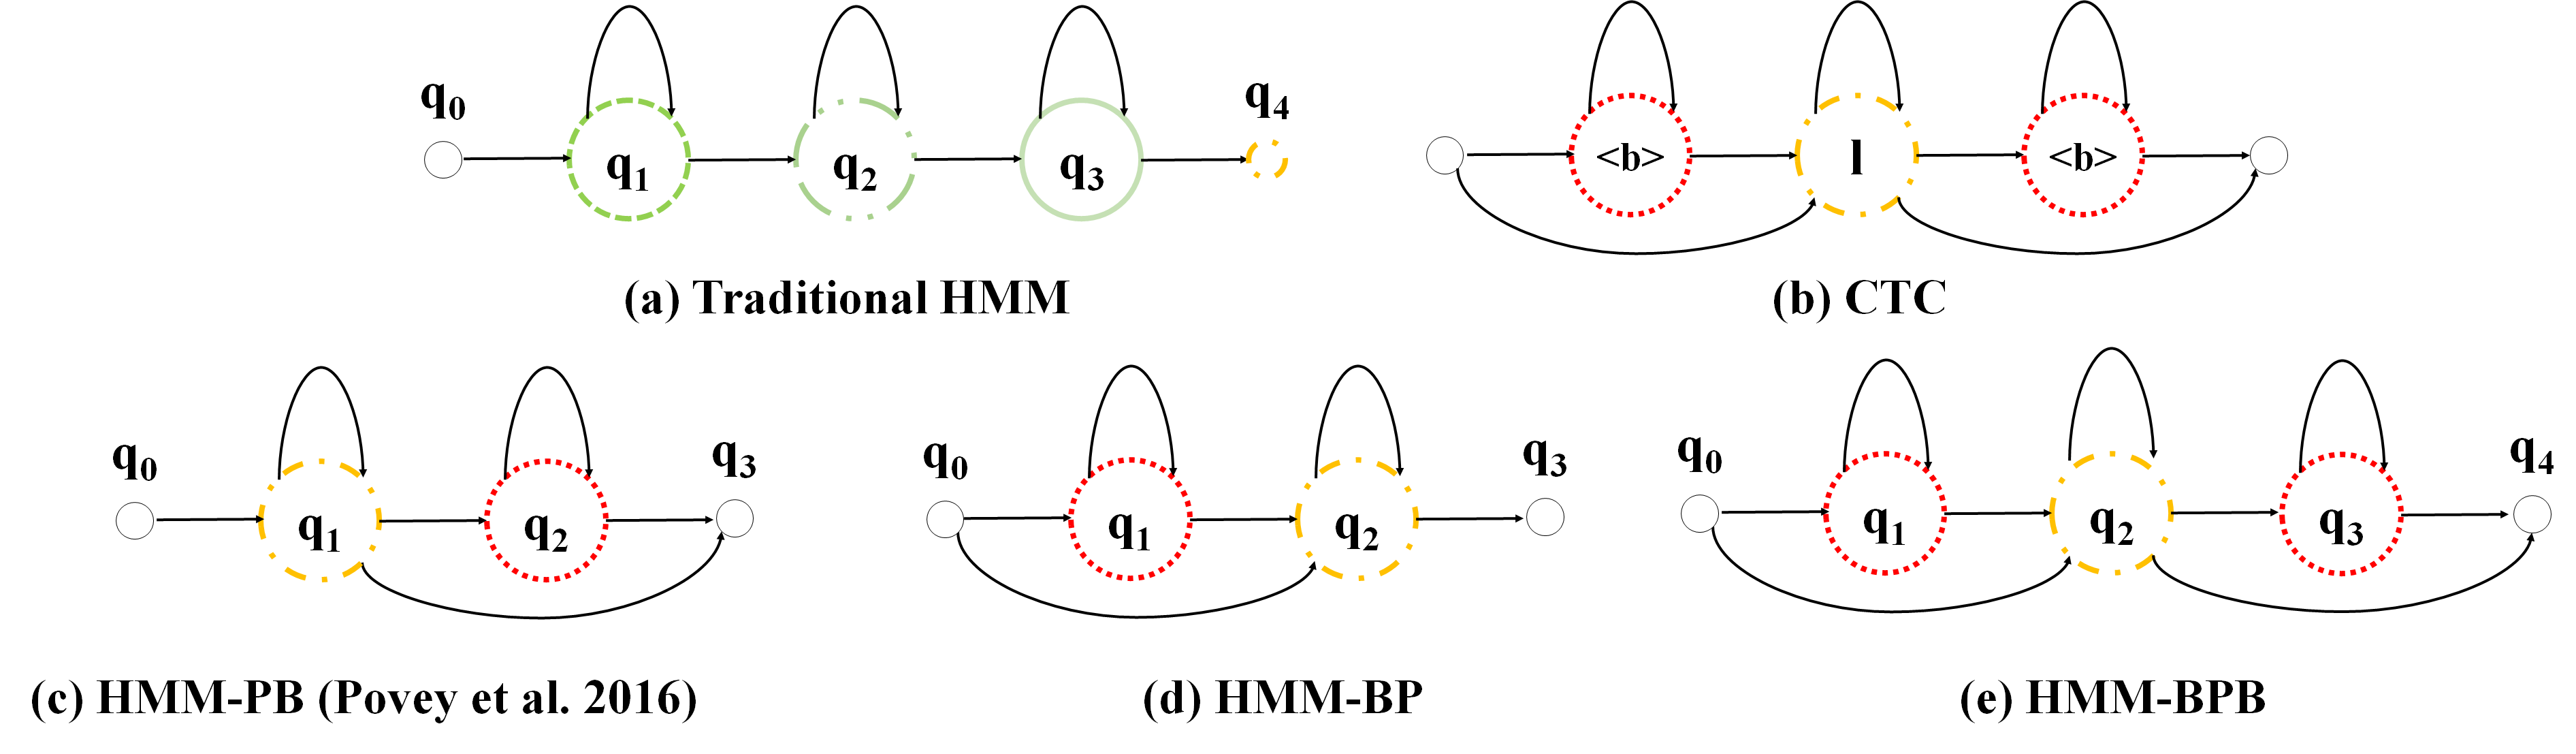
\includegraphics[width=\linewidth]{figure/hmm-topo.png}
    \caption{\it 
    HMM,CTC和本文提出的方法中隐藏状态拓扑结构示意图。 在后面三种拓扑结构中,B指blank HMM状态,P指标签输出HMM状态。每个圆圈代表一个由神经网络建模发射概率的HMM状态。 其中,点划线圆圈表示输出标签建模,如(b)CTC中的l,都各自分配一个特定的模型单元。虚线圆圈表示blank建模,但并不完全相同,如(b)CTC中的<b>是使用公共的blank建模;但(c)中的q2,每个输出标签有独立的blank建模,本文将详细比较不同blank的粒度和拓扑结构所带来的区别。其它实线小圆圈,如(c)中q0、q3,(d)中q0、q3,(e)中q0、q4,代表非发射状态。自循环状态转移表示该状态接受当前状态的重复输出。本文将对这些拓扑结构进行详细比较。
    }
    \label{fig:hmm-topo}
\end{figure*}

\section{基于无词图鉴别性训练模型的标签同步解码}
\label{chap:lsd-lfmmi}

\subsubsection{标签同步解码}
\label{chap:lsd-lsd-hmm}

在GSM中,相邻HMM之间的输出标签也是条件独立的:
\begin{equation} \label{eq:viterbi-blk-hmm}
  \begin{split}
        P(\mathbf{x}|\mathbf{l}) 
        = \prod_{l} P(\mathbf{x}|l) \end{split}
       \end{equation}

类似地,在标签级别上进行的维特比搜索如下所示。
\begin{equation} \label{eq:gsm-dec-lsd}
   \mathbf{w}^* = \mathop{\arg\!\max}\limits_\mathbf{w} \left\{
        P(\mathbf{w})
        \mathop{\max}\limits_{\mathbf{l}_\mathbf{w}}  \prod_{l\in\mathbf{l}_\mathbf{w}} P(\mathbf{x}|l)\right\}
     \end{equation}

在标签中, $P(\mathbf{x}|l)$ 的计算如下所示:
\begin{equation} \label{eq:viterbi-blk-gsm}
  \begin{split}
        P(\mathbf{x}|l)
        = \sum_{\pi:\pi \in L',\mathcal{A}(\pi_{1\mathord{:}T})=l}
          \ \prod_{t=1}^{T} P(\mathbf{x}|\pi_t)P(\pi_t|\pi_{t-1})\\
= \sum_{\pi:\pi \in L',\mathcal{A}(\pi_{1\mathord{:}T})=l}
          \ \prod_{t=1}^{T} P(\pi_t|\mathbf{x})\frac{P(\pi_t|\pi_{t-1})}{P(\pi_t)}
        \end{split}
       \end{equation}  


最近,研究人员们提出了一些新的HMM拓扑结构\cite{povey2016purely,pundak2016lower},它们具有与式\ref{equ:psd-ctc-b}中CTC的$\mathcal{B}$函数类似的一对多映射。以文献\cite{povey2016purely}为例,每个CD音素由两个状态建模,如图~\ref{fig:hmm-topo}(c)所示,且转移概率设置为常数值0.5,因此在式\ref{eq:viterbi-blk-gsm}中可被省略。具体来说,其中一个状态模拟blank建模,如图~\ref{fig:hmm-topo}(b)中的$\tt \langle b \rangle$,另外一个状态则模拟输出标签单元,如图中的$\mathbf{l}$。不同之处在于文献\cite{povey2016purely}中的每个CD音素都保留了自己的blank版本。因此HMM中的状态由标签输出状态或者与CTC类似的blank状态组成。虽然在我们的实验中,这些模型的输出分布比CTC中更平滑,但DSM中提出的公式~(\ref{eq:com-blk-idx}) 和 (\ref{eq:viterbi-blk-ctc})可以被扩展到GSM。


这里提出对神经网络的输出$P(\pi_t|\mathbf{x})$ 进行后处理,其中 $\pi_t $是帧t的推理模型单元。由于这些模型中的模拟blank状态,公式\ref{eq:gsm-dec-lsd}中的维特比束搜索不必包括标签输出候选序列的所有帧。因此,给出某一帧的模型推理分布时,是否从维特比搜索中排除某帧的判决如下:
  \begin{equation} 
       \label{eq:com-blk-idx-gsm}
       \begin{split}
U=\{u:\sum_{l\in L}(y^{u}_{b_l}-y^{u}_{p_l})> \mathcal{T}\}
\end{split}
\end{equation}


其中 $y^{u}_{p_l}$ 是帧u处标签输出状态l的神经网络输出,$y^{u}_{b_l}$ 是对应的blank状态的输出。在第u帧是否有标签输出,是由所有blank状态与标签输出状态的概率差异的总和决定的。T是在开发集中得到的阈值。因此, $P(\mathbf{x}|l)$  的计算可以根据 $\pi\in U$与否分为如下两部分:
\begin{equation} \label{eq:viterbi-blk-hmm2}
  \begin{split}
P(\mathbf{x}|l)
\simeq\sum_{\pi:\pi \in L',\mathcal{A}(\pi_{1\mathord{:}T})=l}
         \{\   \\ %P(b_l|p_l)P(p_l|b_l)
         \prod_{\pi\not\in U}\frac{y_{b_l}^u P(b_l|\mathbf{x})}{P(b_l)} \prod_{\pi\in U}\frac{y_{p_l}^u P(p_l|\mathbf{x})}{P(p_l)}
         \}
         \end{split}
       \end{equation}   


其中第一部分是标签输出状态。在该情况下,每个标签输出均在WFST中进行维特比搜索。而另外一组的blank部分,则假设没有标签输出。不同于CTC,不同标签输出维护自己的blank状态版本。即使是blank帧,也可能包含不同的输出标签信息。因此, $\prod_{\pi\not\in U}\frac{y_{b_l}^u P(b_l|\mathbf{x})}{P(b_l)}$的分数不能被丢弃。上文提出一种高效的算法对这一项进行计算。

这里所提出的后处理可以被视为输出标签概率$P(\pi|\mathbf{x})$的近似,从而使得维特比束搜索得以在标签级别上进行。
我们尝试对FSD和LSD进行对比。

本文提出将特征层面的搜索过程改变为标签层面,即搜索空间是由不同历史的标签组成的,使得解码速率等于标注速率,从而小于特征速率。具体来说,所提出的LSD的解码复杂度如下:
  \begin{equation}
\label{equ:complex-lsd}
\begin{split}
\mathbb{C} \propto (T-|U|)\cdot|L'| \cdot|W|
\end{split}
\end{equation}


其中空白帧的数量 $|U|$,总是接近于T。对比式\ref{equ:complex-fsd}和式(\ref{equ:complex-lsd},FSD得到了很大的加速。这里将FSD和LSD之间的主要区别总结如下:

  不同的信息率。 在FSD中,声学和语言信息均在每帧进行处理,使得二者的处理速率均和声学特征的帧率相同。而在LSD中,声学信息是以声学特征的帧率进行处理的,而语言信息则按声学模型推理的标注速率进行处理。声学和语言信息处理的不同速率去除了大量的搜索冗余。
  可调整的搜索间隔。 在FSD框架下,WFST网络是以等间隔遍历的(即使带有跳帧的深度神经网络在解码\cite{vanhoucke2013multiframe}时是以更长的间隔遍历语言搜索空间,但其间隔仍然是相等的)。 而在LSD中,搜索间隔可通过灵活的自我调整(在不造成性能下降的前提下)来去除blank帧带来的语言搜索空间搜索冗余,这给解码带来了很大的效率提升。



\subsubsection{标签同步解码算法实现}
\label{chap:lsd-lsd-hmm-alg}

用于GSM的标签同步解码算法如算法\ref{code:lsd-gsm-alg}所示。与算法1相比,在每个blank帧中,输出序列可以包含不同的blank单元。因此对相邻的blank帧计算$\prod_{\pi\not\in U}\frac{y_{b_l}^u P(b_l|\mathbf{x})}{P(b_l)}$ 。在非blank帧中,首先将各个blank单元各自累积得到的概率得分分别添加到当前帧的所有候选序列分数中,之后再进行维特比搜索算法。


\begin{algorithm}[ht]
\caption{GSM的标签同步维特比束搜索算法\textcolor[rgb]{0,0.5,0}{(Inputs: 起始节点,结束节点,令牌队列,时间帧)}}
\label{code:lsd-gsm-alg}
\begin{algorithmic}[1]
\Procedure{ LSD for DSM } {S, E, Q, T}
\State $Q \leftarrow S$ \Comment \textcolor[rgb]{0,0.5,0}{起始节点初始化}
\For {each $t\in [1,T]$}    \Comment \textcolor[rgb]{0,0.5,0}{逐帧神经网络前向传播}
\State $F \leftarrow NNPropagate(t)$
\If {!isBlankFrame($F$)}    \Comment \textcolor[rgb]{0,0.5,0}{逐音素解码}
\State  {\color{red}{$F \leftarrow addAccumulatedBlankScore(V,F)$ }}
\State  {\color{red}{$reset(V)$ }}
\State  $Q\leftarrow ViterbiBeamSearch(F, Q)$
\Else         \Comment \textcolor[rgb]{0,0.5,0}{accumulate $\tt blank$ scores}
\State  {\color{red}{$V \leftarrow accumulateBlankScore(V,F)$ }}
\EndIf
\EndFor
\State $\hat B\leftarrow finalTransition(E,S,Q)$ \Comment \textcolor[rgb]{0,0.5,0}{到达结束节点}
\State backtrace($\hat B$)
\EndProcedure
\end{algorithmic}
\end{algorithm}



本文将图\ref{fig:hmm-topo}(d-e)所示的几种改进的HMM拓扑结构应用在了GSM中。具体来讲,在图\ref{fig:hmm-topo}(c)中,每个CD音素都有独立的blank状态,称为CD音素blank (CD phone blank)。为减少模型单元的数量并进一步加快算法速度,将中心音素相同的blank状态绑定在一起,称为音素级blank (phone blank);最后如果绑定所有的blank状态则称作全局bank (global blank)。此外,鉴于标签延迟带来的性能改进\cite{amodei2015deep},图\ref{fig:hmm-topo}(d)中提出HMM-PB模型的延迟标签变种,即HMM-BP。也就是说,模型在确定性标签输出之前输出混淆输出blank。另外,作为对CTC的完整模拟,图\ref{fig:hmm-topo}(e)中提出了HMM-BPB,允许在标签输出前后都存在blank。我们的初步实验结果表明,这两种类型的blank展现出了不同的功能。因此没有将它们绑定在一起。而输出标签单元后面的所有blank则都被绑定在了一起,以减少所需的模型单元数量。

本文在维特比搜索中除了使用传统的束剪枝算法\cite{forney1973viterbi}和直方图剪枝算法\cite{steinbiss1994improvements}(自适应束剪枝\cite{van1996adaptive})之外,提出了另外两种剪枝方法。 在LSD中,blank帧占总帧数的百分比与加速比成正比,而blank帧通过公式进行判定。作为束剪枝算法的变体,这里提出了基于blank帧阈值T的剪枝算法,称为blank剪枝。当阈值T固定时,推理分布的尖峰属性决定了加速比,而尖峰属性显示了神经网络输出分布的置信度。在神经网络的模型训练阶段,本文又提出了基于假设剪枝的熵剪枝算法。 在文献\cite{pereyra2017regularizing}中,作者通过惩罚确定的输出分布来防止过拟合和提高神经网络的泛化能力。受这项工作的启发, 我们在LSD框架中对输出分布的熵进行了控制,作为候选序列的剪枝方法。具体来说,在模型训练中将输出分布的熵添加到负对数似然$\mathcal{L}(\theta)$中,公式如下所示:
  
\begin{equation}
\label{equ:ent-pen-model}
\begin{split}
\mathcal{L}(\theta)= - (\ p_\theta (\pi|\mathbf{x}) - \beta H(p_\theta (\pi|\mathbf{x})\ )
\end{split}
\end{equation}

其中$H(\cdot)$是输出分布 $p_\theta (\pi|\mathbf{x})$的熵,β是正比例因子。与文献\cite{pereyra2017regularizing}不同的是,基于熵剪枝算法的训练目的是最小化模型的原有训练准则以及输出分布的熵。而通常情况下,基于熵剪枝算法是基于一个已经训练好的模型对参数进行微调。在使用新的准则训练之后,LSD框架可在少量性能损失的情况下得以加速。在接下来的实验部分,本文将详细比较这四种剪枝方法。


\section{基于标签同步解码的端到端语音识别}
\label{chap:lsd-e2e}

当前的端到端语音识别系统显示出诸多缺点,在开始使用标签同步解码算法进行优化之前,我们先对这些系统的缺点进行总结。

首先,声学和文本数据并不能够被系统地共同利用,这将导致声学数据的需求量非常大。
目前大多数对文本数据的应用停留于初始化阶段,但却不能系统地使用声学和文本数据,在一个系统框架里。
与之相对,传统基于深度学习的隐马尔可夫训练框架则通过贝叶斯公式,将建模拆分为声学模型,转移模型,词表和语言模型,由此进行模块化的知识源融合。

其次,声学和语言模型总是使用相同的建模单元,而这样的建模单元往往很难兼顾泛化能力和模型性能。音素感知是人类感知的基础单元~\cite{pisoni1985speech}。如果直接使用字符或者词作为建模单元,则并不能建立起这样的建模单元与发音之间的直接关系。这样一些研究忽略了音素这一人类语言中的先验知识。另一方面,使用字符而不是单词作为语言模型的建模单元,同样有损性能~\cite{jozefowicz2016exploring}.

总的来说,端到端系统建立起了与NN-HMM混合系统完全不同的一个模型框架。因此先验知识和之前在语言和声学模型方法的研究很难迁移到这一新的框架中。
%Decoding complexity. In CTC, external language model is used and increases the decoding complexity. In attention-based encoder-decoder, because the prediction in  each step is given by the last prediction, beam search is always taken to reduce the inference bias~\cite{bahdanau2015task}.

\subsection{训练和解码框架}
\label{sec:psd_mod_framework}

之前针对端到端语音识别的研究工作集中在将所有的模型单元融合在一起并进行联合训练和端到端解码。在这项工作中,我们提出了一种模块化的训练策略,以便优化外在知识源分别训练各个子模块的潜力。同时,我们在训练结束后仍然保留端到端解码的优点。图~\ref{fig:psd_mod_framework}显示了这一框架。


\begin{figure}
  \centering
    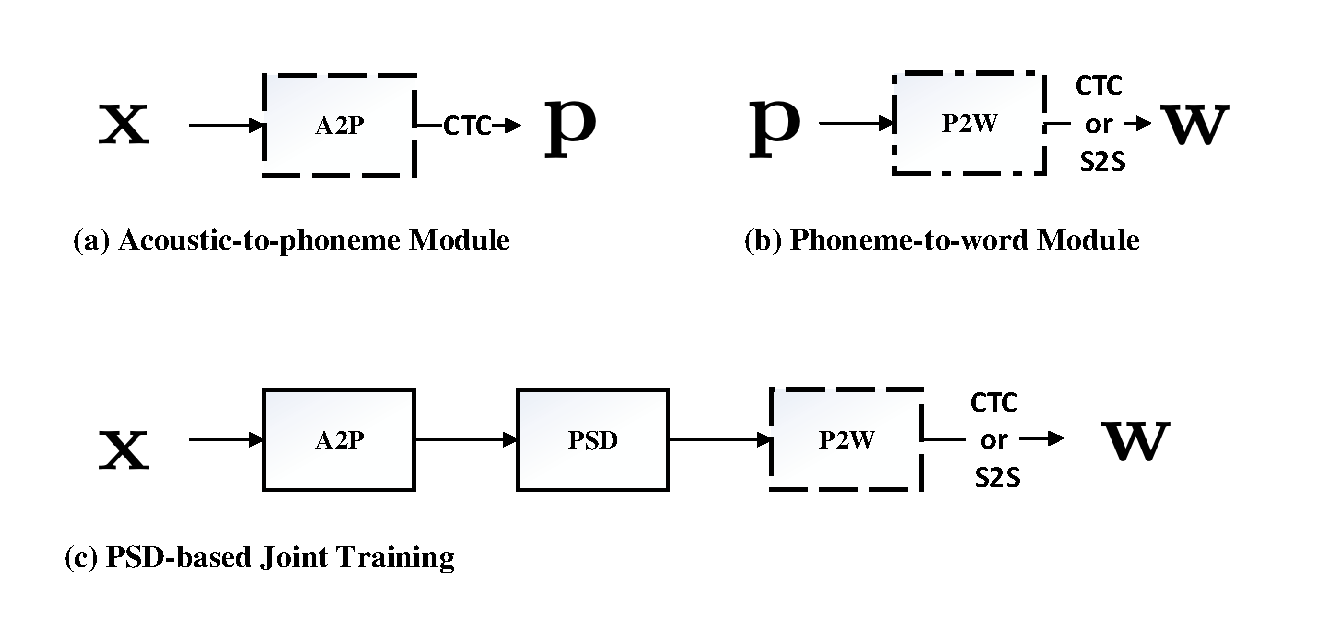
\includegraphics[width=\linewidth]{figure/psd_mod_framework.pdf}
    \caption{\it 模块化训练策略的框架。实线框表示模型参数固定不变的部分。虚线部分和点划线部分分别表示模型参数使用声学或者文本数据进行训练。}
    \label{fig:psd_mod_framework}
\end{figure}

这一端到端词序列识别系统被模块化如下:
\begin{equation}
\label{equ:framework-1}
P(\mathbf{w}|\mathbf{x})\approx\max_{\mathbf{p}} \left[\ P(\mathbf{w}|\mathbf{p}) \cdot P(\mathbf{p}|\mathbf{x})\ \right]
\end{equation}
公式中 $\mathbf{w}$, $\mathbf{p}$ 和 $\mathbf{x}$ 为词序列,音素序列和音频特征序列。
CTC准则被用于训练一个使用声学数据的声学到音素模型 (A2P)  。同时, 我们使用文本数据和CTC或S2S准则训练了一个音素到词语模型。

最终各模块将被融合到一起,成为声学到词语模型 (A2W) ,在联合训练过程中我们使用了音素同步解码算法 (PSD)~\cite{zhc00-chen-tasl2017}。
\begin{equation}
\label{equ:framework-2}
P(\mathbf{w}|\mathbf{x})\approx \max_{\mathbf{p}}\left[\ P(\mathbf{w}|\mathbf{p}) \cdot PSD(\ P(\mathbf{p}|\mathbf{x})\ )\ \right]
\end{equation}
在解码阶段,经过联合训练后的模型将进行端到端推理,因此其复杂度与普通端到端模型相同~\cite{audhkhasi2017direct}。
%As discussed in~\cite{audhkhasi2017direct}, the end-to-end system simplifies the decoding pipeline.  The proposed method still keeps this advantage. 

对于CTC,我们将最佳的推理序列连接起来,得到最终解码序列。对于S2S模型,我们使用维特比束剪枝算法来得到相应结果。这里的端到端模型还可以进一步与外在语言模型相结合以改善性能。在这种情况下,N元语言模型将被编译为词WFST。这种情况下LSD 搜索算法~\cite{zhc00-chen-tasl2017}还可以进一步用于加速系统。


\subsection{模块化}
\label{sec:psd_mod_modu}
由于音素是人类语言重要的先验知识,它建立起了声学和语言之间的关系,因此我们采用它作为理想的建模单元。声学到音素模块使用声学数据进行训练,并预测 $P(\mathbf{p}|\mathbf{x})$ 如图~\ref{fig:psd_mod_framework}(a)所示,其与传统音素CTC建模相同~\cite{miao2015eesen}。注意的是,虽然CTC被用于该项工作,其他传统声学模型同样可以被使用,比如 RNA~\cite{sak2017recurrent} 或者 LF-MMI~\cite{povey2016purely}。

不同于传统模型,我们这里所提出的语言模型使用音素作为输入,推理词序列,即 $P(\mathbf{w}|\mathbf{p})$,也就是一个音素到词的模型,如图~\ref{fig:psd_mod_framework}(b)所示。
另一个主要不同是,P2W模块使用文本和词典,不再需要使用声学数据。
总的来说,P2W模块类似于传统语言模型,除了以下几方面:

i) P2W输入的是音素序列,并隐含进行文本切块。

ii) P2W给定音素序列情况下预测词序列。因此不同于传统的语言模型专注于预测下一个词,在给定前词情况下。P2W实际上得到了更多关于下一个词的信息。因此实验结果显示,P2W的预测准确度明显高于普通的语言模型。

iii) P2W 通过序列级准则进行训练,比如CTC和S2S,这样就能够自动学习到音素和词语之间的对齐关系。


%cmp phone2graphme
我们这里同时引入了一个词边界单元 $\tt wb$ 到音素列表中,以改善文本切块效果。 $\tt wb$ 出现在词语的边界处,比如对词语 ``okay ow k ey'' ,其被修改为``okay ow k ey $\tt wb$''。 这里的想法是使用 $\tt wb$ 作为文本快切分的线索,比如它可以区分一些短词可能是长词前缀的情况。


模块化的优点包括: i) 声学和语言模型都使用了合理的建模单元 ii)系统地结果了声学和文本数据的使用来强化模型训练。


\subsection{标签同步解码}
\label{sec:psd_mod_psd}
标签同步解码在前文已进行了充分介绍,下面我们将使用它,$PSD(\cdot)$ ,作为融合系统中的一个降采样模块,应用在A2P模块上,以减少输入序列的长度。我们这样做的优点包括: i) 更短的序列减轻了LSTM进行时序建模的难度 ii)  加速了联合优化过程 iii) 该方法同时也加速了解码速度~\cite{zhc00-chen-tasl2017}.


\subsection{联合训练}
\label{sec:psd_mod_joint}
最终,所有模块将会被堆叠起来,如图~\ref{fig:psd_mod_framework}(c)所示。声学数据将用来调优该模型。
词语级别的CTC准则使用方法类似于~\cite{soltau2016neural}。
同时S2S被用于词级别的预测。在优化过程中,只有P2W进行联合训练,原因是:i) A2P工作在音素上,通常已经能取得较好性能~\cite{miao2015eesen,sak2015fast}. ii) 固定住A2P使得PSD可以显著减少音频帧数,加快训练速度。经过联合训练后,该模型仍工作在端到端推理上,保留了优点。
%


\section{实验结果}
\label{chap:lsd-exp}

本文实验使用300小时的英语Switchboard数据集作为训练数据\cite{godfrey1992switchboard},使用NIST 2000 CTS作为测试集,对NIST 2000 CTS测试集所包含的switchboard(称为swb)和call-home(称为callhm)两个子集分别进行了评估。在所有实验中使用的是经过工程优化的标准WFST解码器;实验过程中没有生成词图,也没有使用语言模型重打分~\cite{povey2012generating}技术。解码过程中使用在Switchboard和Fisher转录文本上训练的插值的4阶语言模型;在DSM算法验证中,默认使用了经过剪枝的3阶语言模型;在GSM算法验证中,默认使用4阶语言模型,使得结果与文献~\cite{povey2016purely}具有可比性。解码使用的机器配置为Intel(R)Xeon(R)CPU E5-2690 v2 @ 3.00GHz。

本文的DSM实验中,使用具有1.2 M参数的小型CTC模型,使得其适用于嵌入式设备,与文献 \cite{mcgraw2016personalized}可比;使用40维的对数滤波器组特征,特征提取窗宽为25 ms,帧移为10 ms;使用46个单音素作为声学建模单元;声学模型使用3层带有投影层的长短时记忆网络,每层包括400个节点并通过投影层压缩为128个节点~\cite{sak2014long};使用EESEN \cite{miao2016ctc}作为训练工具,训练过程与文献~\cite{miao2015eesen}相似。

本文的GSM实验是在一系列由KALDI流程\cite{povey2011kaldi}训练的基于HMM的大型模型上进行的,这些模型均适用于服务器应用。声学模型建模单元是上下文相关音素。为了提升解码性能~\cite{pundak2016lower,povey2016purely},相对于输入层特征10 ms每帧的帧率,将输出层的输出帧率下降到30 ms每帧。声学模型分别使用每层625个节点的7层时延神经网络(TDNN);以及3层带有投影层的双向长短时记忆网络(BLSTM),其中每层的前向后向层均具有1024个节点,并通过投影层压缩为256个节点。

本文的模块化训练策略的基线系统是一个无模块化训练的端到端系统,也即直接的声学到词语CTC模型,类似于~\cite{audhkhasi2017direct}, 它使用与音素CTC相同的架构,除了在输出层上使用了 30K 大小的词表作为推理单元。它使用了音素CTC进行初始化。

本文实验过程中,使用词错误率(word error rate, WER)来评估不同解码框架下的模型性能,使用搜索过程中的实时率(real time factor (RTF) of the search process, SRTF)和每帧中的活动令牌的平均数量(active tokens, \#AT)来评价搜索速度。在降低帧率的声学模型中,\#AT使用降帧率之前的帧数进行计算;SRTF指解码时间与音频时间的百分比。值得注意的是,这里的解码时间不包括神经网络传播的时间\cite{you2009parallel,hauswald2015sirius}。本文所提出的框架主要加速搜索过程而非神经网络传播,因此不针对不同声学模型的计算速度进行比较,同时这里采用SRTF而不是RTF来评价搜索速度。由于在维特比搜索的搜索迭代过程-即令牌传递算法~\cite{hori2013speech}中,搜索迭代速度与有效令牌的数量相关,因此搜索速度评价指标AT与SRTF总是正相关。为了更加清晰地对比结果,我们还提供了上述指标的相对变化率($\Delta$)作为参考。

\subsection{DSM实验}
\label{exp:dsm}

(1)加速:表1给出了CTC模型下,LSD系统相对FSD系统的加速对比。基于FSD的CTC模型是基线系统。在我们的这项工作中\cite{7736093}曾进一步对比了CTC模型的性能和基于HMM的系统的性能。


\begin{table}[thbp!]
  \caption{\label{tab:exp-lsd-fsd-dsm} {\it LSD versus FSD in DSM}}
  \centerline{
  \begin{tabular}{ m{0.1\columnwidth} ||m {0.08\columnwidth} m {0.08\columnwidth} |m {0.08\columnwidth} m {0.08\columnwidth} m {0.08\columnwidth} m {0.08\columnwidth}}
\toprule
\multirow{3}{0.1\columnwidth}{测试子集  }  &
\multicolumn{2}{c|}{解码性能   }& 
\multicolumn{4}{c}{搜索加速} 
\\
&\multicolumn{2}{c|}{FSD$\mapsto$LSD}&\multicolumn{2}{c}{FSD$\mapsto$LSD}&\multicolumn{2}{c}{FSD$\mapsto$LSD}\\
&WER&$\Delta$(\%)&SRTF&$\Delta$(\%)&\#AT&$\Delta$(\%)\\
\midrule
% https://spetechcular.com/trac/aid201501/wiki/20161011lfmmi-research#modifyHMM
\multirow{1}{0.15\columnwidth}{swb} &  18.7 &+0.5&0.075&-71&2221&-77  \\
%\hline\hline
\multirow{1}{0.15\columnwidth}{callhm} &  33.3 &+0.0&0.073&-70&2211&-77 \\
\bottomrule
\end{tabular}
  }
\end{table}

swb测试子集中,在词错误率相对损失不到0.5%的情况下,与FSD框架相比,LSD框架实现了相对70%以上的SRTF下降(也就是3.4倍的解码加速)。解码加速主要来自于解码过程中减少了搜索迭代次数,解码过程中的活动令牌的数量也体现了这一结果。同时在callhm子集的实验中也能观察到一致的加速效果。

(2)速度鲁棒性:上面的实验解码过程中都使用一个中等大小的语言模型(3阶,3.1 M语言模型),为了测试LSD框架相对于FSD加速效果的鲁棒性(也即对复杂的语言搜索空间下的可扩展性),如图2所示,这里将解码语言模型从2阶变大到4阶[ ],大小从0.2 M变大到4.7 M,使用每帧中的平均活动令牌数(\#AT)来评价解码速度。从图 ~\ref{fig:ctc-dnn-lm-scaleup} 中可以看出,随着语言模型的增大,LSD的\#AT值几乎没有变化,而与此同时,FSD的 \#AT值则明显加速增长。此外,FSD的\#AT值总是远远超过LSD的\#AT值。也就是说,LSD实现的加速对LM搜索空间的增加是鲁棒的,GSM的实验也得出了类似的结论,因此LSD适合应用于更复杂的LM。
 

   \begin{figure}[tbhp!]
   % after de-compress: data/local/lm/sw1_fsh.o3g.kn.gz 76MB data/local/lm/sw1_fsh.o4g.kn.gz 128M
        \centering
        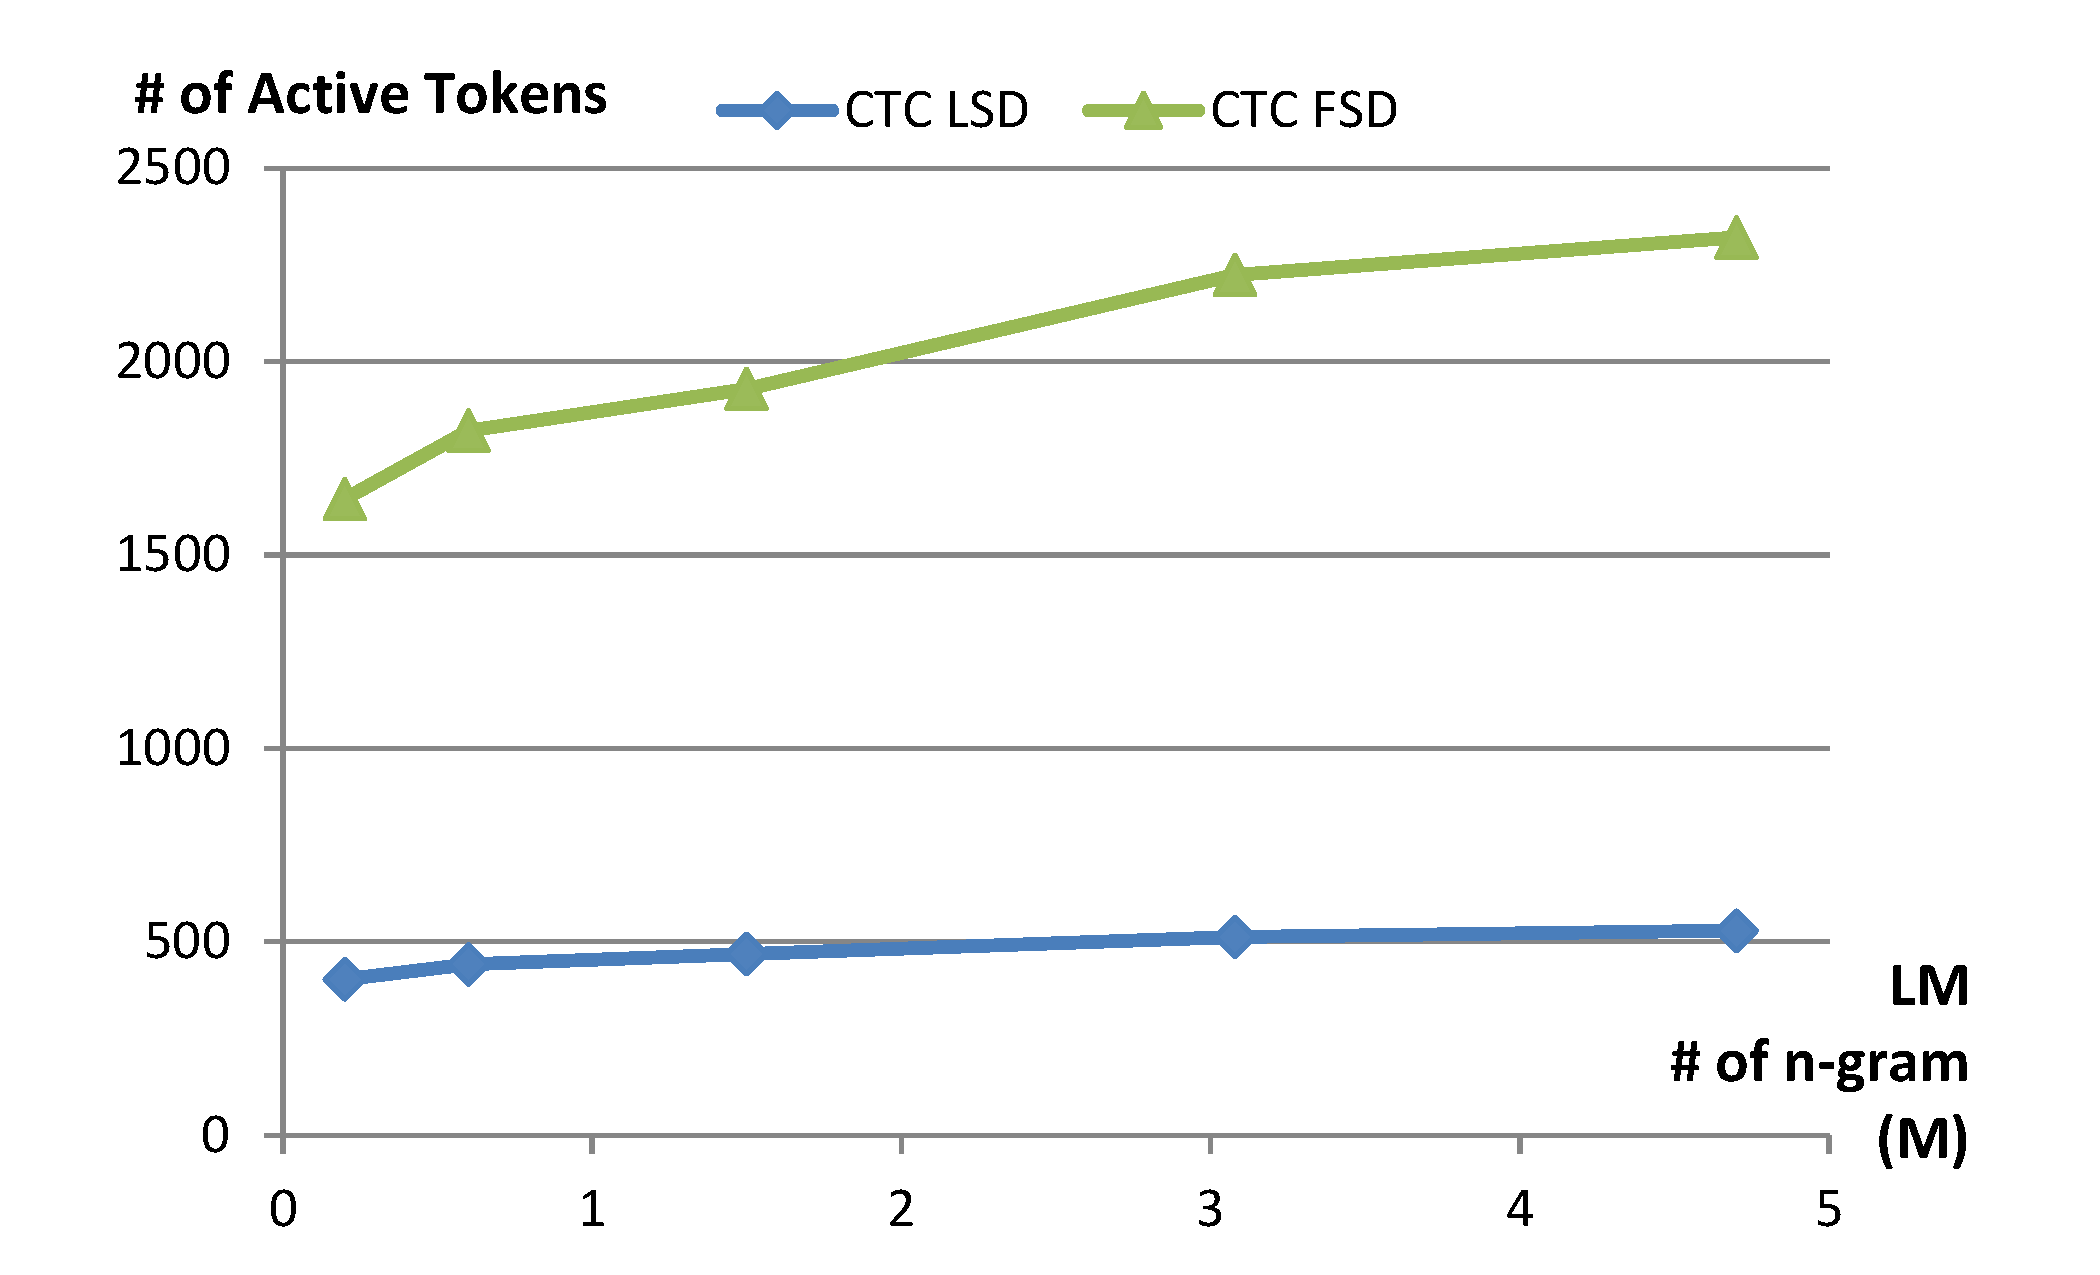
\includegraphics[width=\linewidth]{figure/speed-robust.pdf}
        \caption{{\it LSD和FSD框架中平均活跃令牌数随LM变大的变化趋势。(为清晰起见,这里仅绘制swb子集,calhm子集具有类似变化趋势。)}}
        \label{fig:ctc-dnn-lm-scaleup}
      \end{figure}

(3)结合跳帧方法:该部分对比了跳帧方法下的LSD与FSD框架,实现结果表明可以将跳帧方法与FSD框架进行结合使用。值得注意的是,在后面的实验中,LSD也可以应用于跳帧或降低帧率的GSM声学模型中。

实现方法类似于文献\cite{miao2016simplifying},这里使用LSTM-CTC的2倍跳帧(FS),并且在神经网络后验概率输出层上没有根据原始特征帧率补全后验概率,因此FS也可以加速解码过程;在没有性能损失的情况下,应用于CTC模型的FS可以获得近2倍的解码性能加速。这与文献~\cite{pundak2016lower}中的观察结果一致,并且在LSTM-HMM\cite{miao2016simplifying}和DNN-HMM\cite{vanhoucke2013multiframe}也有类似的结果。LSD可以进一步与FS组合,并且获得更高的效率,即在搜索过程中进一步减少57%(累计为78%)的时间。


\begin{table}[thbp!]
  \caption{\label{tab:exp-cmp-vfr-lsd-dsm} {\it LSD与跳帧方法的对比}}
  \centerline{
  \begin{tabular}{ m{0.1\columnwidth} ||m {0.08\columnwidth} m {0.08\columnwidth} |m {0.08\columnwidth}  m {0.08\columnwidth} m {0.20\columnwidth} }
\toprule
\multirow{3}{0.1\columnwidth}{测试子集}  &
\multicolumn{2}{c|}{解码性能  }& 
\multicolumn{3}{c}{搜索加速} 
\\
&\multicolumn{2}{c|}{FSD$\mapsto$FS+LSD}&\multicolumn{3}{c}{FSD$\mapsto$FS$\mapsto$FS+LSD}\\
&WER&$\Delta$(\%)&SRTF&$\Delta_{FS}$&$\Delta_{+LSD} $ ($\sum$)\\
\midrule
% https://spetechcular.com/trac/aid201501/wiki/20161011lfmmi-research#modifyHMM
\multirow{1}{0.15\columnwidth}{swb} &  18.7 &-1.6&0.075&-48&-57 (-78)  \\
\multirow{1}{0.15\columnwidth}{callhm} &  33.3 &-0.6&0.073&-47&-57 (-77) \\
\bottomrule
\end{tabular}
  }
\end{table}

(4)候选序列剪枝:图\ref{fig:prune-wer-at-dsm}比较了本文提出的LSD框架与传统的剪枝技术,即束剪枝(表示为beam)和直方图剪枝(表示为histogram)。 在LSD中,通过调整公式\ref{eq:com-blk-idx}和\ref{eq:com-blk-idx-gsm}中定义的T来调整加速比和性能,这也可以被视为另一种候选序列剪枝方法(表示为blank)。 上文中提出的基于熵剪枝算法表示为entropy。
 

\begin{figure}[tbhp!]
   % after de-compress: data/local/lm/sw1_fsh.o3g.kn.gz 76MB data/local/lm/sw1_fsh.o4g.kn.gz 128M
        \centering
        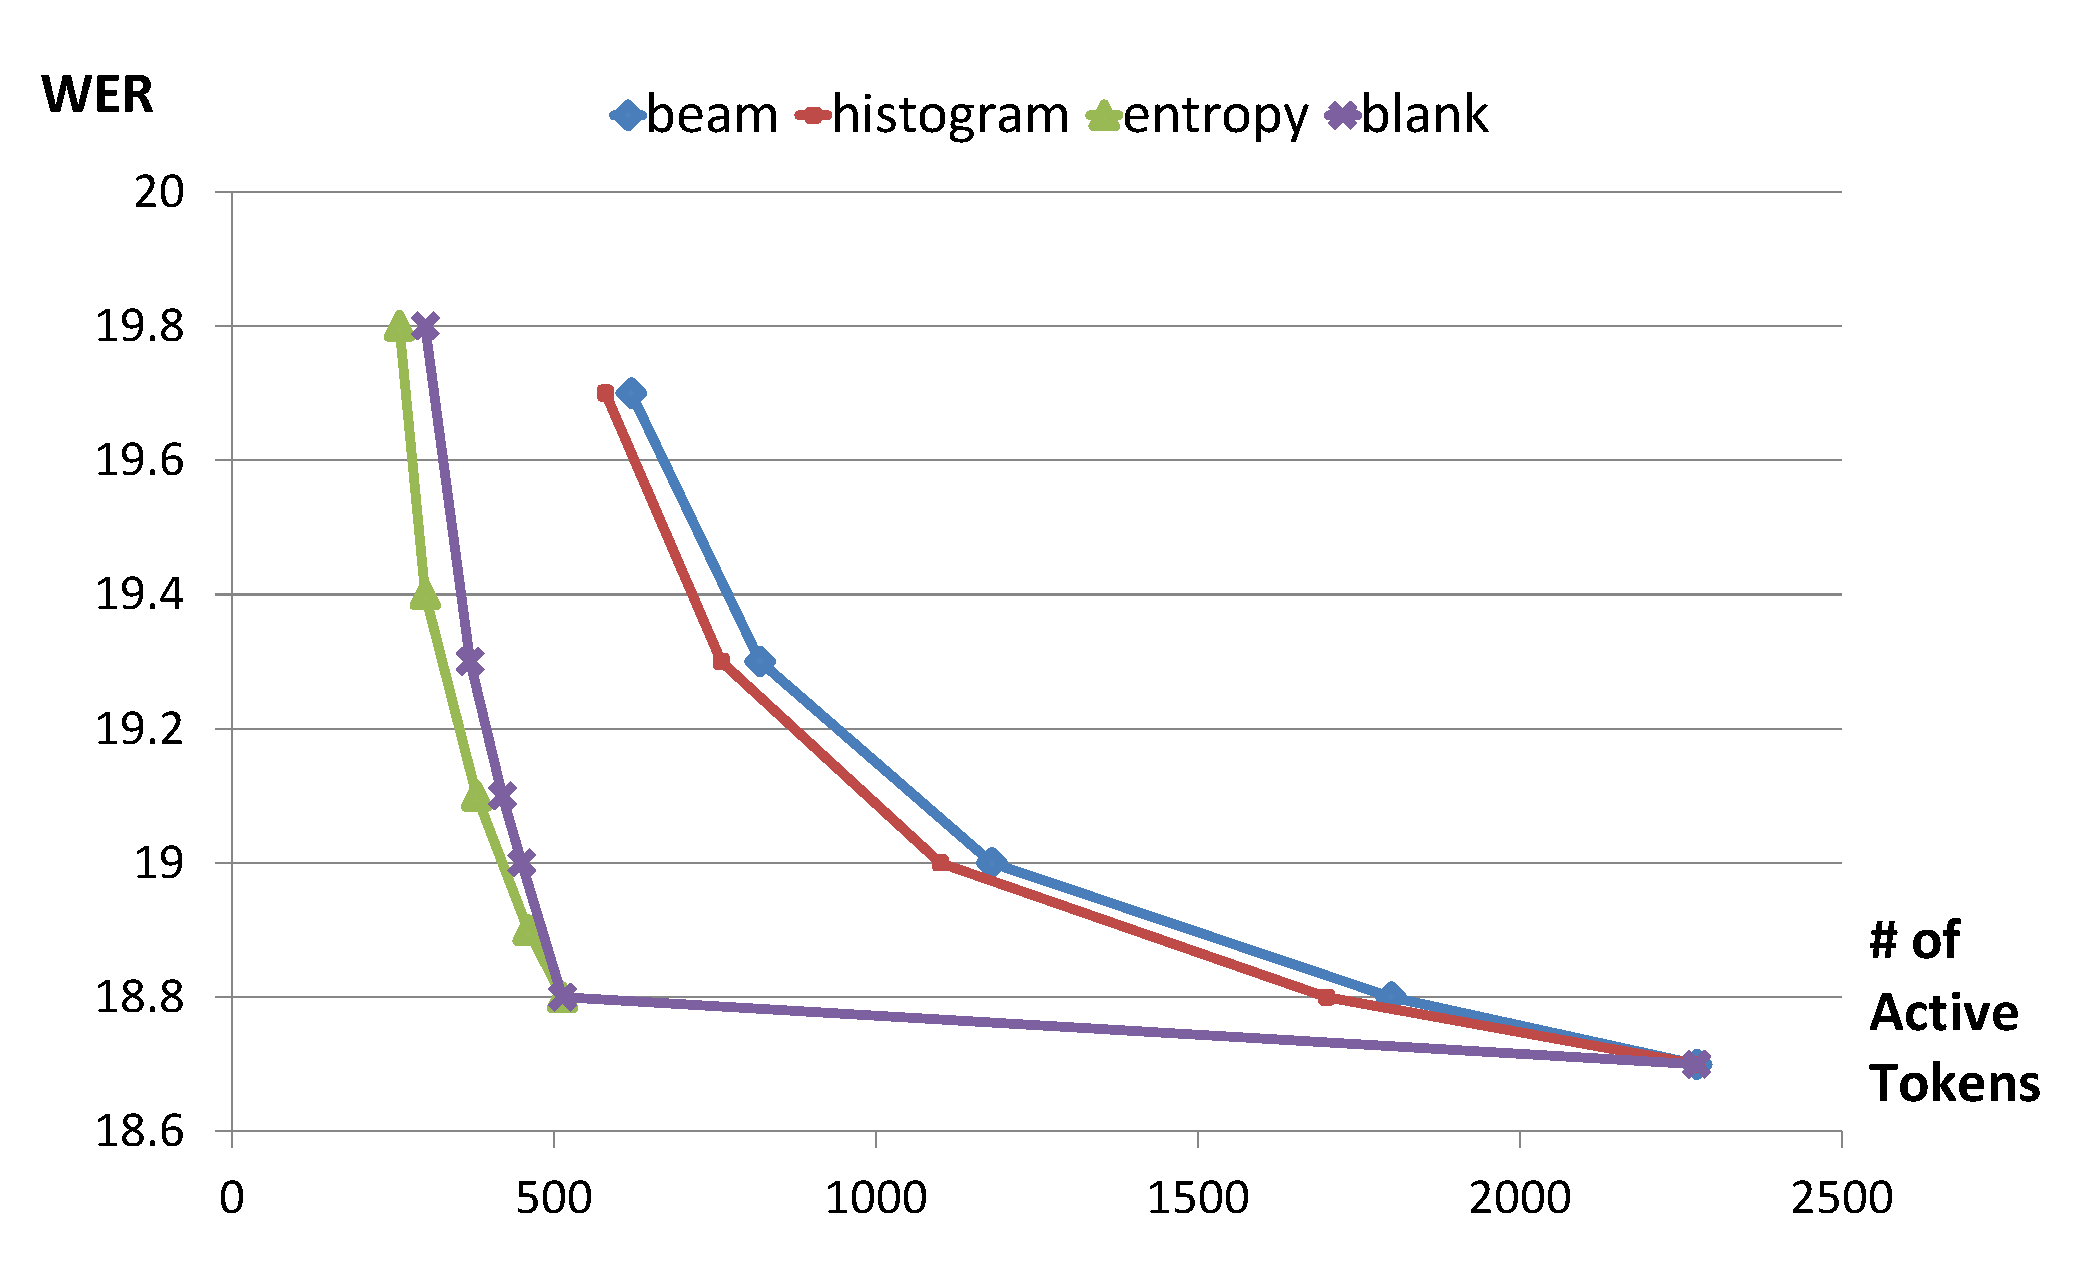
\includegraphics[width=\linewidth]{figure/prune-wer-at-dsm.pdf}
        \caption{{\it 对于swb子集,CTC中,使用不同剪枝技术时WER随平均活跃令牌数的变化趋势。calhm子集结果类似 }} %The number of average active tokens is obtained by the original frame rate before reduction.
        \label{fig:prune-wer-at-dsm}
      \end{figure}


从图中可以看出,基于LSD的方法,entropy和blank,与基于FSD的方法beam和histogram相比保持显著优势。其原因在于,基于FSD的候选序列剪枝对所有候选序列进行统一处理,而相反,LSD框架可以看作是将候选序列划分为特征级别和标签级别。因此,如公式\ref{eq:ctc-dec-lsd}及公式\ref{eq:com-blk-idx}所示,LSD框架中,可以在特征层和标签层进行剪枝。也即,基于LSD的候选序列剪枝方法受益于将搜索过程从特征层转移到标签层。

另外结果显示,为了加速解码,两种框架中的方法都会降低解码性能,而且基于LSD的方法解码性能下降更严重。如前所述,基于FSD和LSD的方法之间的关键区别在于后者的阈值T仅与特征层上的候选序列剪枝有关。特征层候选序列剪枝的加速比几乎是固定的,在不损害性能的情况下,70-80%的候选序列可以被剪枝掉。图\ref{fig:prune-wer-at-dsm}中blank曲线具有明显的拐点(\#AT = 513,WER = 18.8),也源于同样的原因。在图的最右侧,未进行特征层剪枝时,blank曲线最终达到了与基于FSD的方法的同一点。由于上面讨论的明显拐点及固定加速比,可以很容易得到等式\ref{eq:ctc-dec-lsd}中的阈值T。此外,特征层的entropy和blank剪枝可以进一步与标签层的beam和histogram方法相结合,以得到最佳的解码加速效果。为了使对比更加清晰,图中没有给出融合系统的曲线。

最后,entropy的效率略高于blank(相对约10%)。我们认为原因在于神经网络中剪枝能更好地利用神经网络输出分布中的信息,并且产生更好的精度和效率。而blank剪枝则仅利用了输出分布中的最佳分数而未使用整个分布的信息。

\subsection{GSM实验}
\label{exp:gsm}
(1)在各种模型和准则中的应用:LSD应用于生成式序列模型(GSM)时,本文使用了多种不同的神经网络模型结构和模型训练准则进行对比;默认使用上下文相关的音素作为模型建模单元。表\ref{tab:exp-lsd-fsd-gsm}给出了在NIST 2000 CTS测试集合上的结果。总体而言,LSD框架也可以取得比较显著的解码加速,但是与表\ref{tab:exp-lsd-fsd-dsm}中的结果相比,解码加速性能变差。这是因为FSD基线的帧率已经降低到原来的1/3\cite{pundak2016lower}(类似前文中帧率改变技术可以与提出的LSD框架结合)。而且与表\ref{tab:exp-cmp-vfr-lsd-dsm}相比,加速比也略小,原因是这些模型的推理分布概率不像CTC那样尖锐。如何在GSM中获取更尖锐的推理分布概率将在该部分的(2)和(3)中进行讨论。

具体地,如表~\ref{tab:exp-lsd-fsd-gsm}所示,第一行列出了文献\cite{pundak2016lower}中提出的低帧率模型(LFR)的结果;第二行是使用LF-MMI准则\cite{povey2016purely}训练出来的结果,显示出比LFR更快的搜索速度;此外,还可以看到从FSD到LSD,基于 LF-MMI准则训练的模型可以取得更快的加速。与文献\cite{paulik2015improvements}中观察到的类似,这都源于序列区分性训练准则得到的模型相对于交叉熵准则训练的模型有更尖锐的输出概率分布。第三行表示为+ sMBR,是在LF-MMI模型的基础上,使用基于LM的sMBR准则微调模型参数得到的结果;第四、五行列出了基于增强的MMI\cite{povey2008boosted}及sMBR准则变体的无需词图的区分性训练准则取得的结果,分别表示为LF-bMMI和LF-sMBR。可以观察到,本文提出的LSD框架在以上模型和准则中可以取得一致的解码加速。另外我们还使用了BLSTM模型,也都取得了相似结果。


     \begin{table}[thbp!]
        \caption{\label{tab:exp-lsd-fsd-gsm} {\it  LSD与FSD在不同的GSM模型上的性能和速度比较}}
        \centerline{
\begin{tabular}{ m{0.1\columnwidth} |m {0.15\columnwidth} ||m {0.06\columnwidth} m {0.06\columnwidth} |m {0.06\columnwidth} m {0.06\columnwidth} m {0.06\columnwidth} m {0.06\columnwidth}}
      \toprule
      \multirow{3}{0.1\columnwidth}{模型}  &
      \multirow{3}{0.15\columnwidth}{准则} & 
      \multicolumn{2}{c|}{性能 }& 
      \multicolumn{4}{c}{速度} 
      \\
      &&\multicolumn{2}{c|}{FSD$\mapsto$LSD}&\multicolumn{2}{c}{FSD$\mapsto$LSD}&\multicolumn{2}{c}{FSD$\mapsto$LSD}\\
      &&WER&$\Delta$(\%)&SRTF&$\Delta$(\%)&\#AT&$\Delta$(\%)\\
      \midrule
      \multirow{6}{0.1\columnwidth}{TDNN} & CE  & 17.8&+1.0&0.16&-38&3705&-41 \\
      & LF-MMI &15.6 &+1.0&0.13&-43 &  3386&-45\\
      %local/chain/compare_wer_general.sh tdnn_7h_sp_smbr
      & \ \ +sMBR &15.4 &+1.0&0.12&-41 & 3295 & -43 \\
      %\cline{2-5} local/chain/compare_wer_general.sh tdnn_7h_b0.1_s1_1_sp
      & LF-bMMI &15.0 &+1.0&0.11&-42 & 3198 & -44 \\
      %\cline{2-5}
      & LF-sMBR &15.3 &+1.0&0.12&-41 & 3288 & -44 \\
      \midrule
      %local/chain/compare_wer_general.sh blstm_6h_sp
      \multirow{2}{0.1\columnwidth}{BLSTM}& LF-MMI &15.2 &+1.0&0.12&-44&3290 &-47 \\
      %local/chain/compare_wer_general.sh blstm_6h_b0.2_s2_3_sp
      & LF-bMMI &14.3 &+1.0&0.11&-43& 3205&-45 \\
      \bottomrule
      %\hline\hline
      \end{tabular}
        }
      \end{table}



(2)候选序列剪枝:如图\ref{fig:prune-wer-at-gsm}所示,我们在生成式序列模型下进行了一系列候选序列剪枝相关的实验,其变化趋势类似于DSM中的结果,读者可以参考那里的讨论。与图\ref{fig:prune-wer-at-dsm}中一个区别在于,beam,histogram,blank,entropy在图\ref{fig:prune-wer-at-gsm}中的最左边位于相同点,这表明在降低帧率的情况下,特征层候选序列剪枝的最大比例较小。 然而,在解码性能的WER达到最佳时,仍然有接近两倍的解码加速。



 
\begin{figure}[tbhp!]
   % after de-compress: data/local/lm/sw1_fsh.o3g.kn.gz 76MB data/local/lm/sw1_fsh.o4g.kn.gz 128M
        \centering
        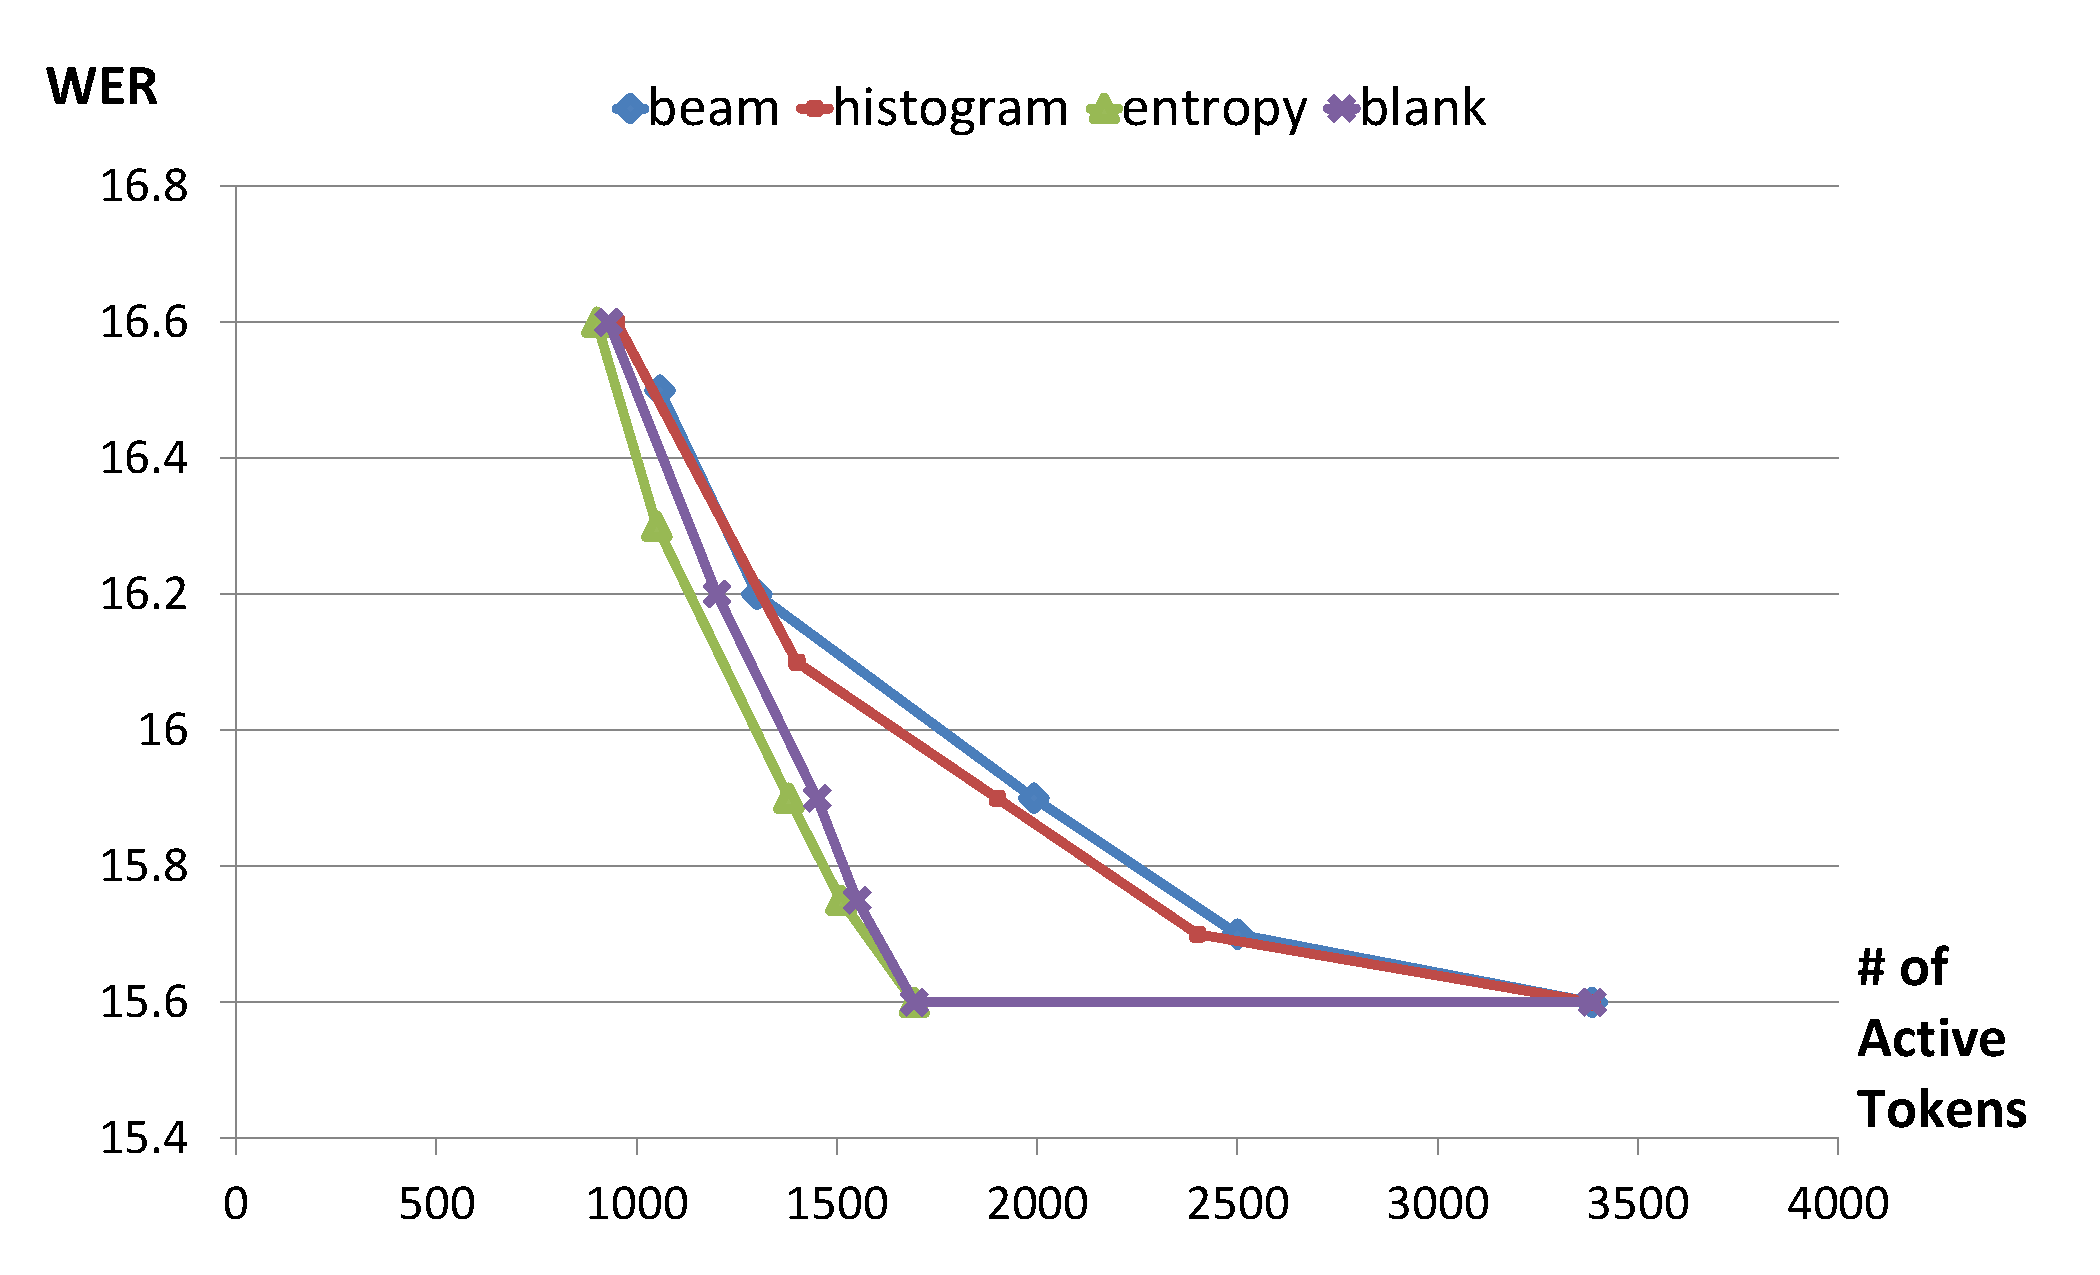
\includegraphics[width=\linewidth]{figure/prune-wer-at-gsm.pdf}
        \caption{{\it  LF-MMI中,使用不同剪枝技术时WER随平均活跃令牌数的变化趋势  }}
        \label{fig:prune-wer-at-gsm}
      \end{figure}
   
(3)进一步设计:本节将对比前文中讨论的各种转移模型,以及由此获得的效率的进一步提高。该部分所有实验均在LF-MMI准则上进行,但实验结论可以扩展到其它神经网络和训练准则上。 


     \begin{table}[thbp!]
        \caption{\label{tab:exp-blk-gran-gsm} {\it 生成式序列模型中的blank粒度}}
        \centerline{
    \begin{tabular}{ m{0.1\columnwidth} |m {0.15\columnwidth} ||m {0.06\columnwidth} m {0.06\columnwidth} |m {0.06\columnwidth} m {0.06\columnwidth} m {0.06\columnwidth} m {0.06\columnwidth}}
      \toprule
      \multirow{3}{0.1\columnwidth}{系统}  &
      \multirow{3}{0.15\columnwidth}{$\tt blank$} & 
      \multicolumn{2}{c|}{性能 }& 
      \multicolumn{4}{c}{速度} 
      \\
      &&\multicolumn{2}{c|}{FSD$\mapsto$LSD}&\multicolumn{2}{c}{FSD$\mapsto$LSD}&\multicolumn{2}{c}{FSD$\mapsto$LSD}\\
      &&WER&$\Delta$(\%)&SRTF&$\Delta$(\%)&\#AT&$\Delta$(\%)\\
%      \hline \hline
      %\multirow{2}{0.13\columnwidth}{CE} & $\times$ & & & \\
%      \cline{2-5}
%      & $\surd$ & & & \\
%      \hline\hline
      %\multirow{2}{0.15\columnwidth}{sMBR} & $\times$ & & & \\
%      \cline{2-5}
%      & $\surd$ & & & \\
      \midrule
      \multirow{3}{0.15\columnwidth}{TDNN LF-MMI} &  CD phone &15.6 &+1.0&0.13&-43&3386&-45 \\
      & phone &15.7 &+0.9&0.09&-47&2785& -50\\
      % local/chain/run_tdnn_7h_inphone.sh
      % ref: https://spetechcular.com/trac/asr/milestone/report-yby23-2016-11-06
      %local/chain/compare_wer_general.sh tdnn_7h_mhmm_BP_sp
      & global &16.8 &+0.8&0.09&-49&2512& -54 \\
      \bottomrule
%      \hline\hline
      \end{tabular}
        }
    \end{table}

表~\ref{tab:exp-blk-topo-gsm}中列出了不同blank粒度的对比结果,即上下文相关的音素blank (CD phone blank),音素blank (phone blank)和全局blank (global blank)。与CD phone blank基线相比,phone blank在取得近似的解码性能的同时,实现了显著的搜索过程加速;这里搜索加速主要源于较少的模型建模单元,即模型状态数从6K减少到3K。此外,从表中可以看出,global blank会带来明显的性能下降;global blank需要足够的数据来覆盖不同相邻音素之间的上下文环境(我们认为这也是CTC准则在这个语料库中表现更差的原因之一);CD phone blank可以缓解blank训练数据不足的问题,但会导致搜索速度变慢;因此,绑定中心音素相同的CD phone blank在加速搜索过程的同时,也可以更好地建模blank模型;因此,phone blank是解码性能和搜索速度之间的最佳平衡。此外,从表\ref{tab:exp-blk-topo-gsm}中可以看出,在LSD框架下,较少的模型单元可以持续带来明显的搜索过程时间缩短:43%→47%→49%。最后,phone blank是基于GSM的LSD框架的最佳选择。


     \begin{table}[thbp!]
        \caption{\label{tab:exp-blk-topo-gsm} {\it 生成式序列模型中的blank拓扑结构}}
        \centerline{
        \begin{tabular}{ m{0.1\columnwidth} |m {0.1\columnwidth} ||m {0.06\columnwidth} m {0.06\columnwidth} |m {0.06\columnwidth} m {0.06\columnwidth} m {0.06\columnwidth} m {0.06\columnwidth}}
      \toprule
      \multirow{3}{0.1\columnwidth}{测试集}  &
      \multirow{3}{0.1\columnwidth}{拓扑} & 
      \multicolumn{2}{c|}{性能 }& 
      \multicolumn{4}{c}{速度} 
      \\
      &&\multicolumn{2}{c|}{FSD$\mapsto$LSD}&\multicolumn{2}{c}{FSD$\mapsto$LSD}&\multicolumn{2}{c}{FSD$\mapsto$LSD}\\
      &&WER&$\Delta$(\%)&SRTF&$\Delta$(\%)&\#AT&$\Delta$(\%)\\
%      \hline \hline
      %\multirow{2}{0.13\columnwidth}{CE} & $\times$ & & & \\
%      \cline{2-5}
%      & $\surd$ & & & \\
%      \hline\hline
      %\multirow{2}{0.15\columnwidth}{sMBR} & $\times$ & & & \\
%      \cline{2-5}
%      & $\surd$ & & & \\
      \midrule
      % https://spetechcular.com/trac/aid201501/wiki/20161011lfmmi-research#modifyHMM
      \multirow{3}{0.15\columnwidth}{TDNN LF-MMI} &  PB &15.6 &+1.0&0.13&-43&3386&-45  \\
      & BP & 15.6 &+1.0&0.13&-46&3392&-49 \\
      %sharper than BPgB
      %& gBPB & 10.4&+1.0&&&& \\
      & BPB & 15.6 &+1.0&0.13&-47&3388&-51 \\
      \bottomrule
%      \hline\hline
      \end{tabular}
        }
    \end{table}

表\ref{tab:exp-blk-topo-gsm}对比了前文提出的不同HMM拓扑结构。在FSD框架下,所有拓扑结构都有相似的解码结果和相同的搜索速度。对比前两行可以看出,与基线PB拓扑结构相比,在LSD框架下, BP可以获得更大的搜索加速。我们认为这个更优的搜索加速源于标签延迟现象,类似于文献\cite{amodei2015deep}中观察到的现象,这使得模型能更可靠地推断标签输出状态并减少混淆。因此,这能带来更尖锐的输出分布。从表中还可以看出,BPB拓扑结构可以进一步改善搜素速度;一些解码路径的例子也表明这种拓扑结构可以使每个上下文相关的隐马尔可夫模型输出更多的blank状态。最后,与表2中CTC的结果相比,GSM中LSD框架能减少49%的搜索时间。

\subsection{标签同步解码在模块化训练中的应用}
\label{exp:psd_mod}

表\ref{tab:exp-module}针对各个模块的验证集(CV)上的性能进行了比较。加粗的系统将在后续中进行使用。

\begin{table}[thbp!]
  \caption{\label{tab:exp-module} {\it  各个模块的性能比较 }}
  %\vspace{1mm}
  \centerline{
    \begin{tabular}{c c c c||m{0.15\columnwidth}}
      \hline
      模块  & 模型 & 推理单元 & 词边界 & PER/WER CV (\%) \\
      \hline \hline
      \multirow{2}{0.08\columnwidth}{A2P}& \multirow{2}{0.08\columnwidth}{CTC} & \multirow{2}{0.15\columnwidth}{phoneme} & $\times$& 13.0 \\
      &  &  & $\surd$& {\bf 12.0} \\
      \hline\hline
      \multirow{4}{0.08\columnwidth}{P2W}& \multirow{2}{0.08\columnwidth}{CTC}  &\multirow{2}{0.1\columnwidth}{word}   & $\times$  &16.0 \\
      &  &  & $\surd$  &{\bf 4.3} \\
      \cline{2-5}
      & \multirow{2}{0.08\columnwidth}{S2S}  & \multirow{2}{0.1\columnwidth}{word}  & $\times$  & 13.9 \\
      &  &  & $\surd$  & {\bf 2.8} \\
      \hline
    \end{tabular}
  }
\end{table}

在A2P中,音素CTC的识别性能与~\cite{graves2006connectionist}中一致。 
%add wb didnt affect result, 
引入的$\tt wb$ 并不影响ASR性能。 
%the slight imp because Error rate of A2P phoneme with wb includes wb token
该系统中轻微的性能改善来自统计PER时包含了 $\tt wb$这一单元。而进一步统计 $\tt wb$ 的预测准则显示其低于 4\%。

在P2W模块中,CTC和S2S都进行了比较。在不包含 $\tt wb$ 情况下,二者的性能都不好。正如前文所讨论的, $\tt wb$ 可以提供音素序列切分的线索,因此CTC和S2S在包含$\tt wb$ 之后都得到了提升。
S2S一致地由于CTC,这是由于CTC中的CIA被去除,使建模能力得到增强~\cite{chan2016end}。 
不同于传统的语言模型,这里不适用PPL作为准则,原因是本系统自动推理出音素与词之间的对齐关系,并使用序列准则进行训练。

%add blk modeling, both good
%bold taken for the latter exp


在第二部分中,我们比较了联合训练之后的结果,显示在表~\ref{tab:exp-joint}中。
%Table~\ref{tab:exp-joint} shows the results.
%proposed method versus the hybrid system and several end-to-end systems. 
%Notably, all systems utilize the Switchboard corpus without external sources.
为了更好地支撑这些结果,我们与近期在同一数据集上的公开结果进行比较~\cite{audhkhasi2017direct}。 
这里的不同实验配置包括:i) 添加i-vector自适应 ii)使用BLSTM iii) 语言模型使用了Fisher数据集。
因此本实验系统与~\cite{audhkhasi2017direct}中的系统包含相对 20-30\%的差距。 

\begin{table}[thbp!]
  \caption{\label{tab:exp-joint} {\it  针对是否包含模块化训练的性能比较 }}
  \centerline{
    \begin{tabular}{c |c |c m{0.15\columnwidth}||c c}
      \hline
       & E2E& \multicolumn{2}{c||}{Modularization } & \multicolumn{2}{c}{WER (\%)}\\
       Name &  Opt. & A2P&P2W & swbd & callhm \\
      \hline \hline
      %/speechlab/users/mkh96/asr/baseline/swbd/lstm/exp/plstm5/decode/eval2000_0.0833/score_13_0.0/eval2000.ctm.swbd.filt.sys
      %/fgfs/users/zhc00/works/ctc/allctc/amctc/ceam
      %exp/plstm5/decode_lang_decode_sw1_tg/eval2000_0.0833/score_12_0.0/eval2000.ctm.swbd.filt.sys
      CD-phone CE & $\times$ & HMM & WFST  &  14.9 & 27.6 \\
      %exp/plstm_ctc5/decode_sw1_tg/eval2000_0.6/
      CI-phone CTC & $\times$ & CTC & WFST  & 19.4 & 33.5 \\
      \hline\hline
       %Word CTC& $\surd$ & n/a & n/a  & 35.7 & 47.1 \\   
      \multirow{1}{0.17\columnwidth}{Word CTC}&$\surd$ & n/a & n/a  & 29.6 & 41.7 \\         
      \hline\hline
      %exp/swb.plstm_ctc5_wb.f.d2w.2d.train_tr90.3d2.tr.lstm_l2_c384_p256/decode.final.nnet/eval2000/ctm.swbd.filt.sys
      %exp/swb.plstm_ctc5_wb.f.d2w.2d.train_tr90.3h4.tr.lstm_l2_c700_p256/decode.final.nnet/eval2000/
      \multirow{2}{0.17\columnwidth}{Mod. CTC}&$\surd$ & CTC & CTC  & 24.9 & 36.5 \\   
      &$\surd$ & CTC & \ \ \ \ +WFST  & 23.0 & 35.1 \\ 
      \hline
       \multirow{1}{0.17\columnwidth}{Mod. S2S}&$\surd$ & CTC & S2S  & 31.2 & 40.5 \\   
      \hline
    \end{tabular}
  }
\end{table}

基线的混合系统 (CD-phone CE) 和音素 CTC (CI-phone CTC)系统罗列于第一和二行。他们都是通过WFST联合解码得到的。
%
CI-phone CTC 的性能比CD-phone CE差~\footnote{在更多数据情况下,CTC 性能比传统系统好~\cite{sak2015fast}。我们之前的研究也显示同样的结论 \cite{zhc00-chen-tasl2017}}, 这里的性能差距类似于之前在~\cite{audhkhasi2017direct}中的发现。
%Meanwhile, the gap between CD-phone CE and CI-phone CTC in this work is also similar to that in~\cite{audhkhasi2017direct}.
%
直接进行 A2W建模的 CTC (Word CTC)模型在第三行。它包含了音素模型初始化,但不包含GloVe初始化~\cite{audhkhasi2017direct}。
这里的性能明显差于 CI-phone CTC。该系统为不带有模块预训练的基线系统。

我们所提出的模块化训练系统 (Mod. CTC) 在第四行。
我们使用了基于标签同步解码的联合训练,该工作的具体效果将在表~\ref{tab:exp-psd} 中继续讨论。
Mod. CTC  显著改善了基线系统的性能。更好的性能来自: i) 得益于模块化和初始化所带来的更快和更好的模型收敛 ii) 更易于分别使用声学和文本数据来融合传统的声学和语音模型训练技术。

表~\ref{tab:exp-psd}显示了引入PSD算法的重要性。所有的结果都是基于一张 Titan GPU所得到。 ``fr./s.''表示每秒钟所处理的声学帧数。这里的训练加速来自两方面: i)PSD减少了后续P2W需要处理的序列长度 ii) 由于序列长度有所减小,更多的序列可以被载入GPU显存,由此可以加速并行计算。
同时,性能也有所改善。我们认为改善的结果来自于序列长度的缩短。虽然我们使用LSTM,但模型仍然很难记忆很长的序列。但是对于A2W建模,需要记忆的历史显著长于传统的 CI-phone CTC 或者混合系统。在其他一些研究中~\cite{chan2016end}也有类似的现象,而这些研究通过金字塔式的降帧率来缓解该问题。PSD是解决该问题的另一种思路。

%cmp several tricks:
%\begin{itemize}
%\item Table~\ref{tab:exp-psd} shows with or without PSD. 4 titan. speedup from larger streams \& PSD reduce seq len
%\item Table~\ref{tab:exp-add-text} shows the effect of  adding text data
%\end{itemize}

\begin{table}[thbp!]
  \caption{\label{tab:exp-psd} {\it  是否包含PSD情况下的模型性能和训练速度 }}
  \centerline{
    \begin{tabular}{c c||c c| c c}
      \hline
        && \multicolumn{2}{c|}{训练速度} &  \multicolumn{2}{c}{WER (\%)} \\
       Name & PSD & Seq./GPU&  fr./s. & swbd & callhm \\
      \hline \hline
      %exp/swb.plstm_ctc5.d2w.1a.train_tr90.3d3.tr.lstm_l2_c384_p256/log/train_nnet.log
     \multirow{2}{0.2\columnwidth}{Mod. CTC} & $\times$ &5 & 1027 & 32.0 & 42.5 \\
      %exp/swb.plstm_ctc5_wb.f.d2w.2d.train_tr90.3d2.tr.lstm_l2_c384_p256/log/iter05.tr.log
        & $\surd$ &{\bf 30} & {\bf 5851} & {\bf 24.9} &{\bf 36.5}  \\
      \hline
    \end{tabular}
  }
\end{table}

为了减轻CTC的CIA假设对模型性能所带来影响,我们实验了以下一些方案。
首先,一个从N元语言模型得到的WFST被用于与模型一起进行联合解码,其结果显示在表~\ref{tab:exp-joint}的第五行。该系统得到了一定性能提升。由此第2行与第5行的性能差距被缩减到少于 15\%。
%
另一种方法是使用S2S来代替CTC。我们提出的基于模块化训练的S2S系统 (Mod. S2S) 在表~\ref{tab:exp-joint}中最后一行。不同于在表~\ref{tab:exp-module}中的现象,S2S系统并未得到性能改善。通过进一步分析解码结果,我们发现S2S很易于受到音素识别错误的影响。经过联合优化后,S2S并不能恢复这些错误,这项观察同样见于其他研究~\cite{prabhavalkar2017comparison}。
%Especially, the acoustic signal is filled with much more noises than the phoneme sequences. 
在我们的研究中尚未包含字符级别的建模系统,原因是字符对于声学和语言建模的难度都比较大,如前文所述,音素和词语对本文的建模更加直接。



\section{本章小结}
\label{chap:lsd-sum}

在本章中,我们针对语音识别和端到端建模的忒单,提出了一系列标签同步解码算法,其通过一系列方法使得搜索解码过程从逐帧同步变为标签同步,这包括使用高效的blank结构和后处理方法。该文提出的一系列通用方法在隐马尔科夫模型和连接时序模型上得到了验证。同时该章节还介绍了将标签同步算法应用于序列到序列的端到端模型的方案。在实验部分,该章节系统一方面取得大幅度语音识别解码速度改善,另一方面在端到端建模上取得了更快和更好的模型收敛和模型准确度。
